\section{Energy consumption patterns}\label{sec:observations}
We perform a set of static experiments to determine which factors affect the energy consumption
patterns of programs. Our aim is to determine whether there are cases where using all available
resources is not optimal, and whether optimizing for energy-efficiency always correlates with
optimizing for runtime. We do this to gain insight that informs the design process of the dynamic
adaptation algorithm in Section~\ref{sec:implementation}.

Presumably, using all available resources of a system does not necessarily lead to the lowest energy
consumption. Energy consumption patterns of programs are influenced by a wide range of factors, such
as algorithm implementation, workload behaviour, and hardware characteristics. To illustrate this we
investigate the effect these factors have on the energy consumption pattern of the N-body,
nine-point stencil, and matrix multiplication algorithms. Within the context of data-parallel
programming, these algorithms provide an interesting mix of CPU-bound and memory-bound applications.

Benchmarks are conducted on an Intel Xeon E-2378 server, maintained by the Radboud University. The
system is accessible through Slurm, and contains a single 8 core 16 thread CPU, running at a base
clock of 2.60GHz. The CPU has 16MB of level three cache, and the system itself provides 32GB of RAM.

\begin{figure*}[!ht]
    \centering
    \begin{subfigure}{0.33\linewidth}
        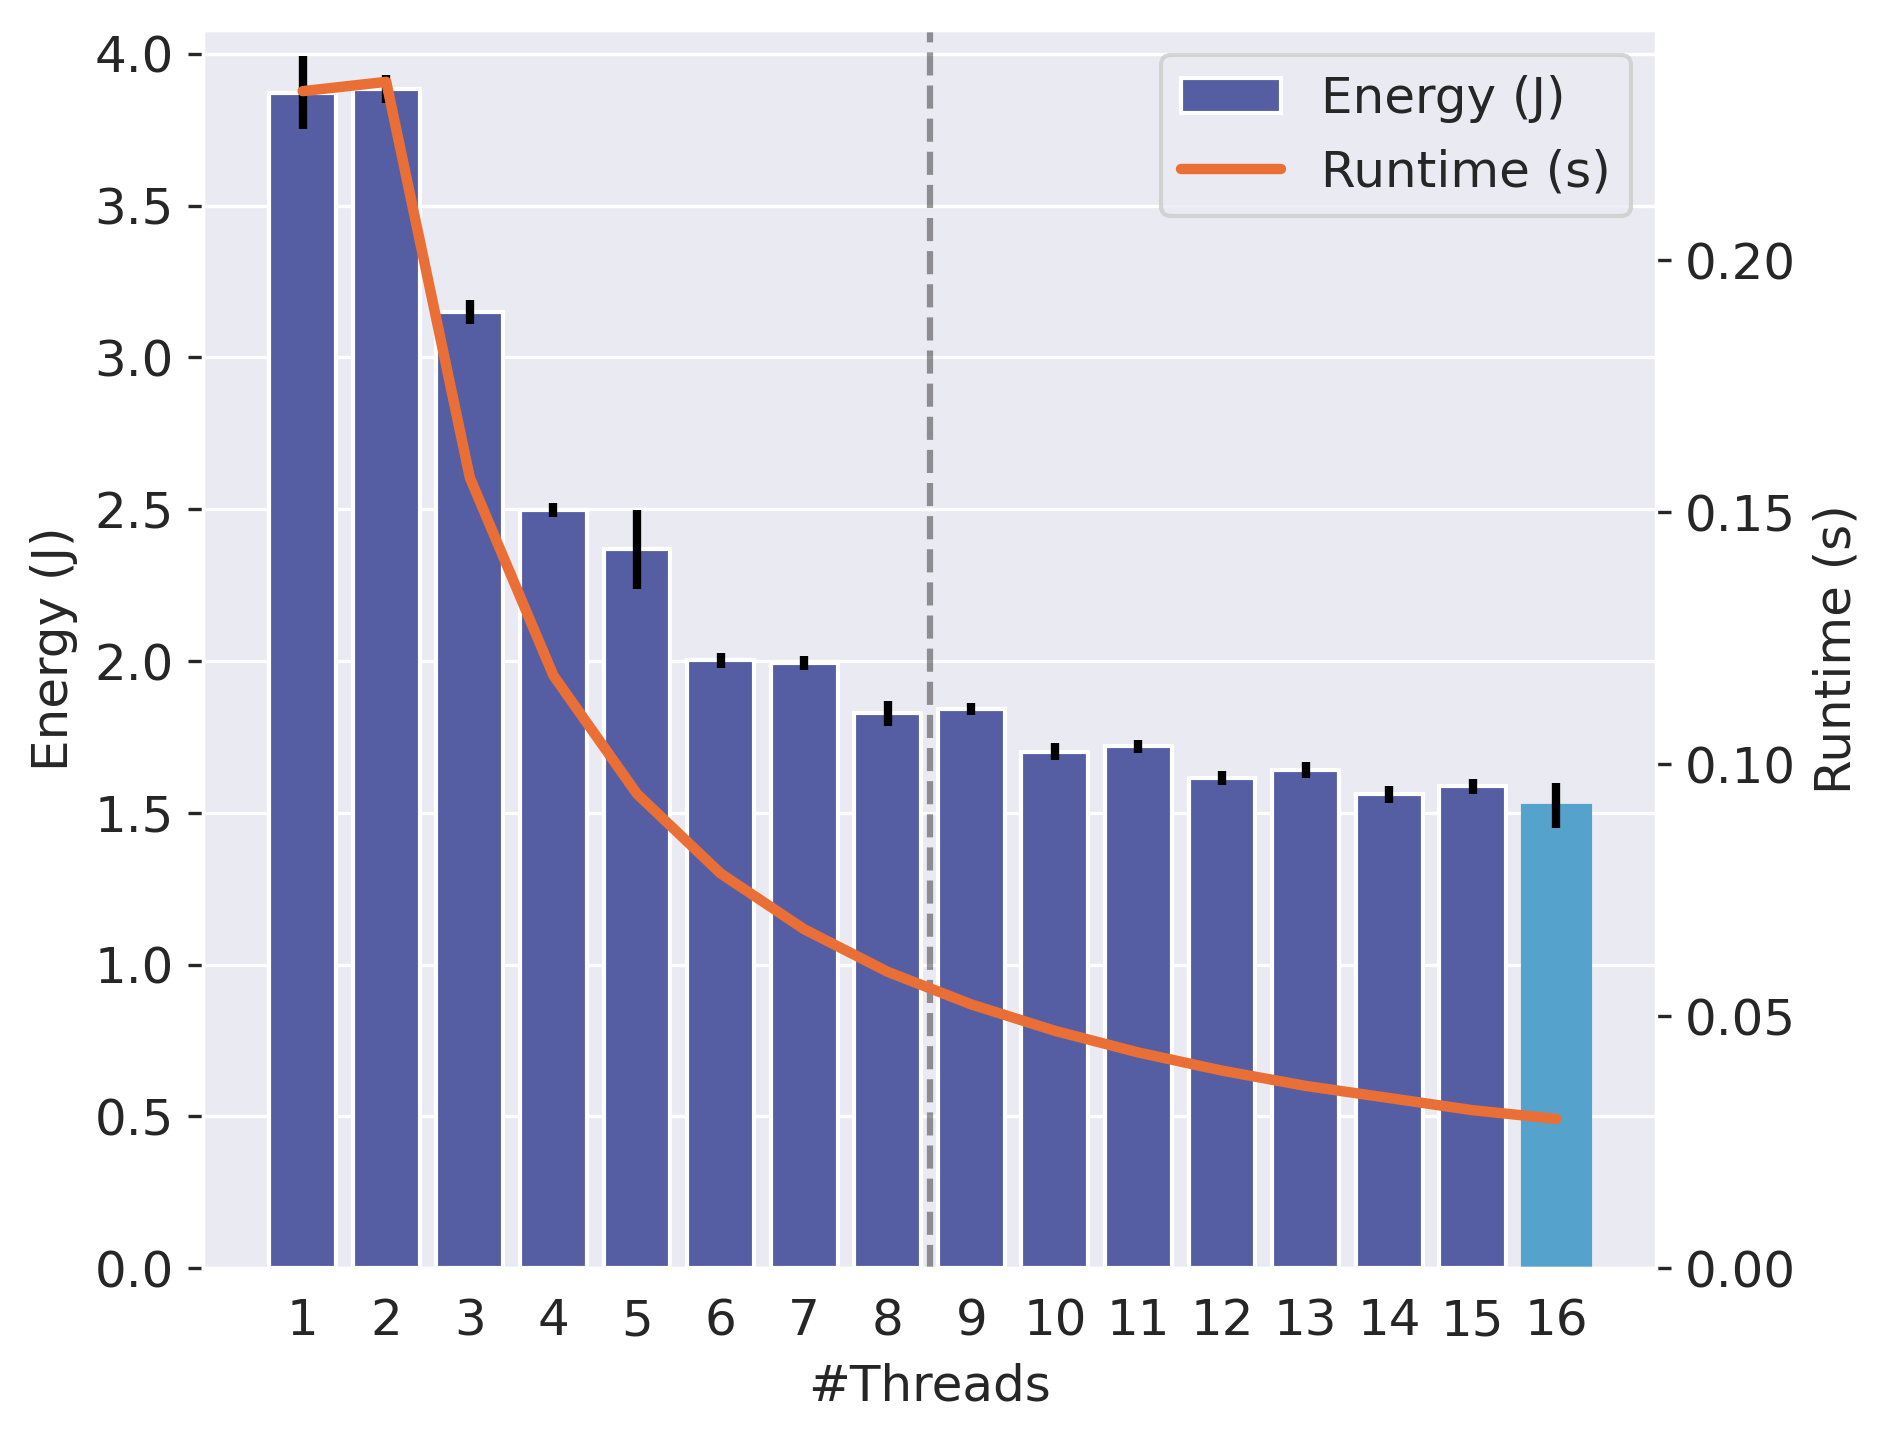
\includegraphics[width=\linewidth,alt={
            Chart showing energy consumption and runtime across different numbers of threads. The
            x-axis represents the number of threads from 1 to 16. The left y-axis shows bars
            indicating energy consumption in joules. The right y-axis shows an orange line
            indicating the runtime in seconds. Energy consumption peaks at two threads, and steadily
            decreases until roughly eight threads, after which it plateaus and reaches a minimum at
            16 threads. Runtime peaks at two threads, and gradually decreases until it reaches the
            minimum at 16 threads.
        }]{images/nbody_10000.png}
        \caption{$10000$ elements.}
        \label{fig:nbody1}
    \end{subfigure}%
    \begin{subfigure}{0.33\linewidth}
        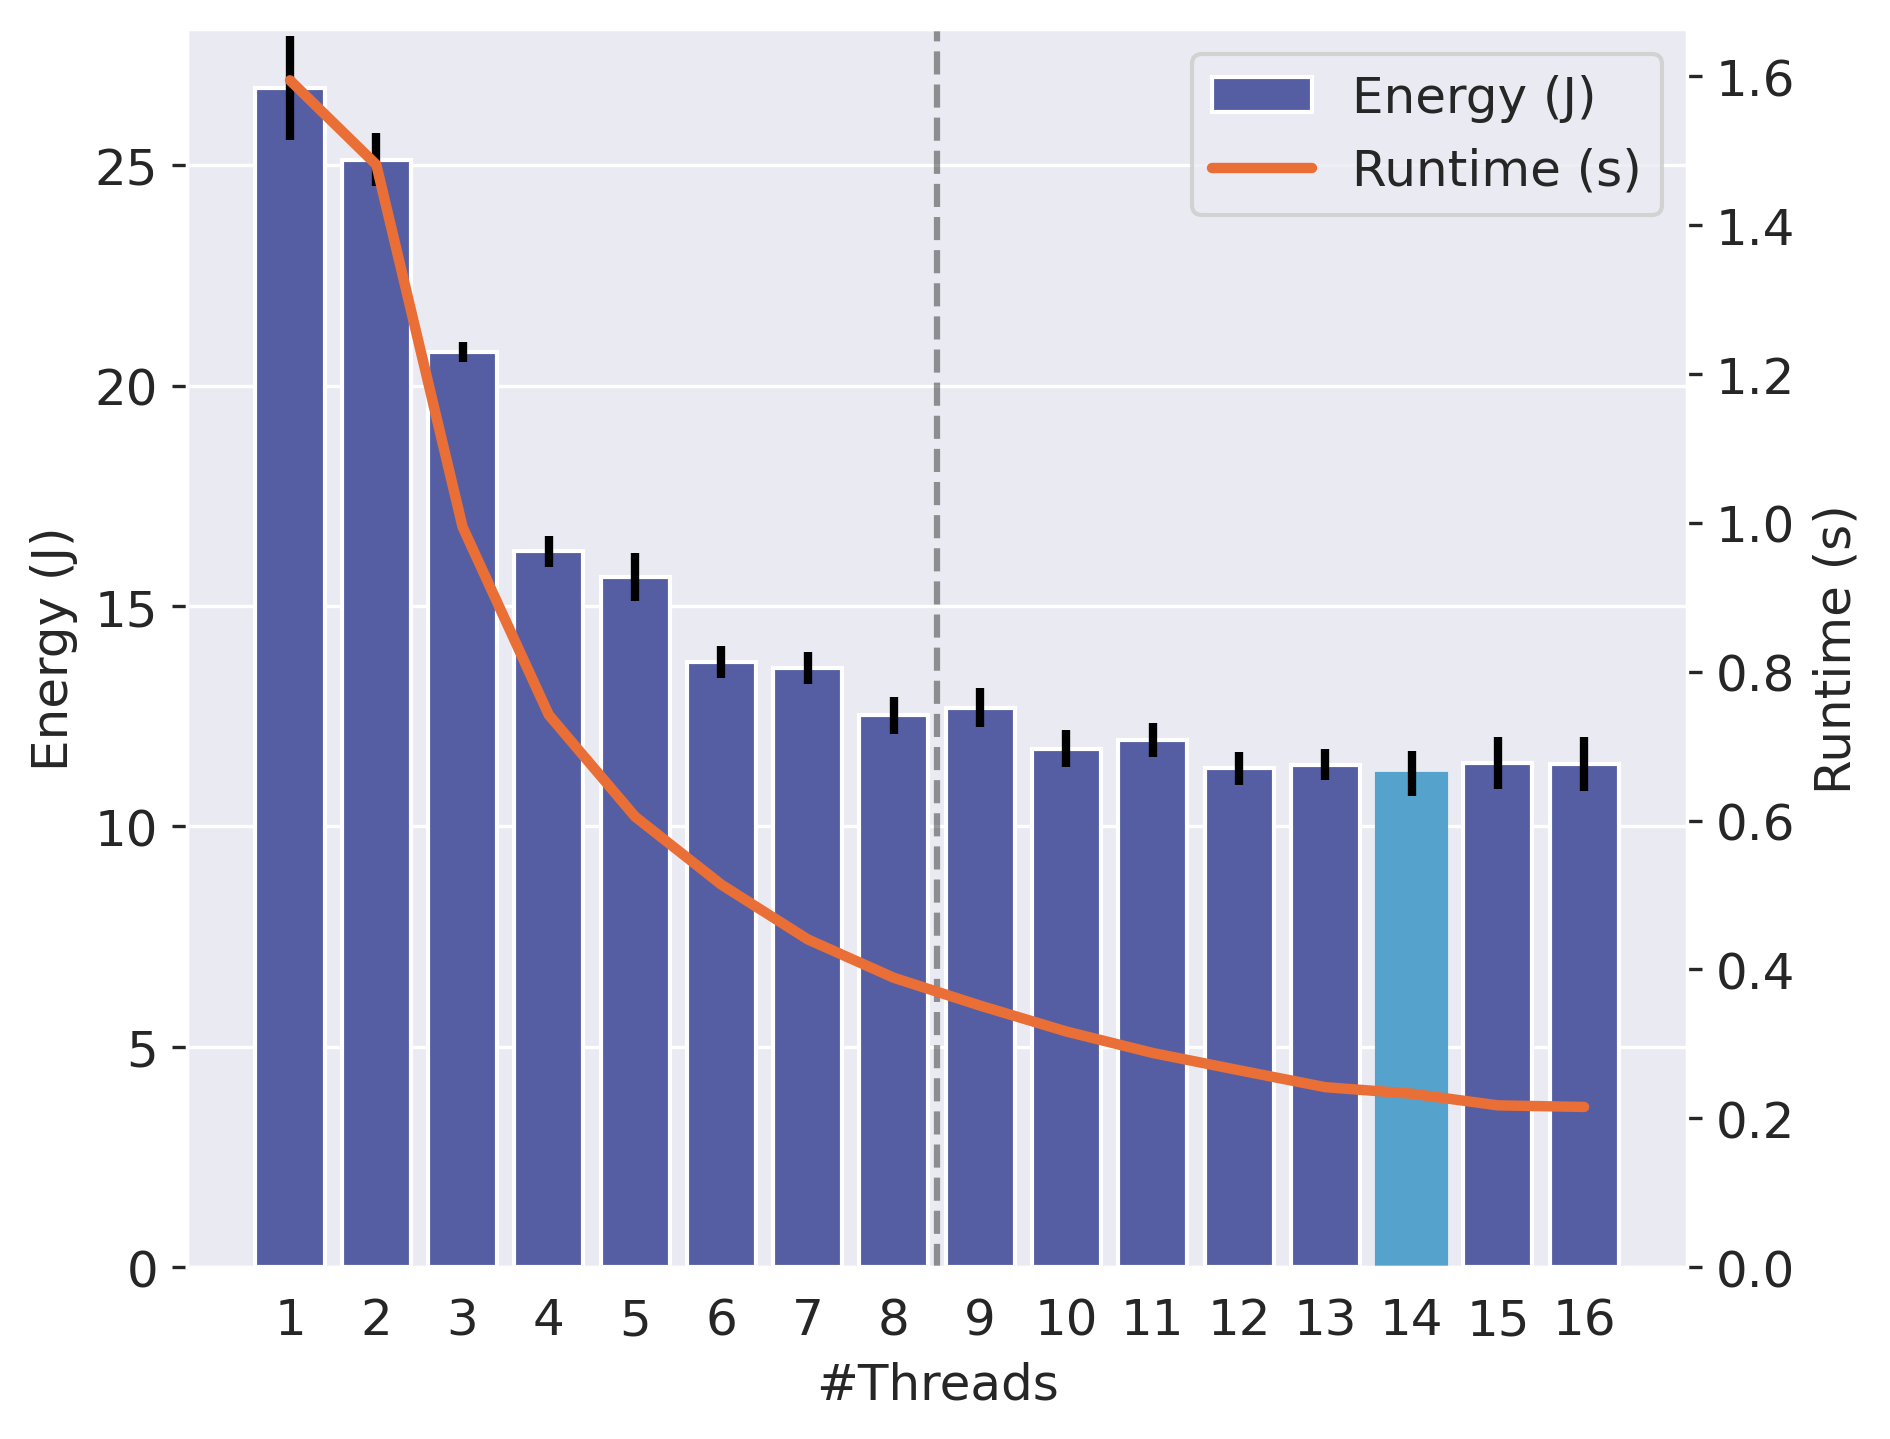
\includegraphics[width=\linewidth,alt={
            Chart showing energy consumption and runtime across different numbers of threads. The
            x-axis represents the number of threads from 1 to 16. The left y-axis shows bars
            indicating energy consumption in joules. The right y-axis shows an orange line
            indicating the runtime in seconds. Energy consumption peaks at one thread, and steadily
            decreases until roughly eight threads, after which it plateaus and reaches a minimum at
            14 threads. Runtime peaks at one thread, and gradually decreases until it plateaus
            around 14 threads.
        }]{images/nbody_25000.png}
        \caption{$25000$ elements.}
        \label{fig:nbody2}
    \end{subfigure}%
    \begin{subfigure}{0.33\linewidth}
        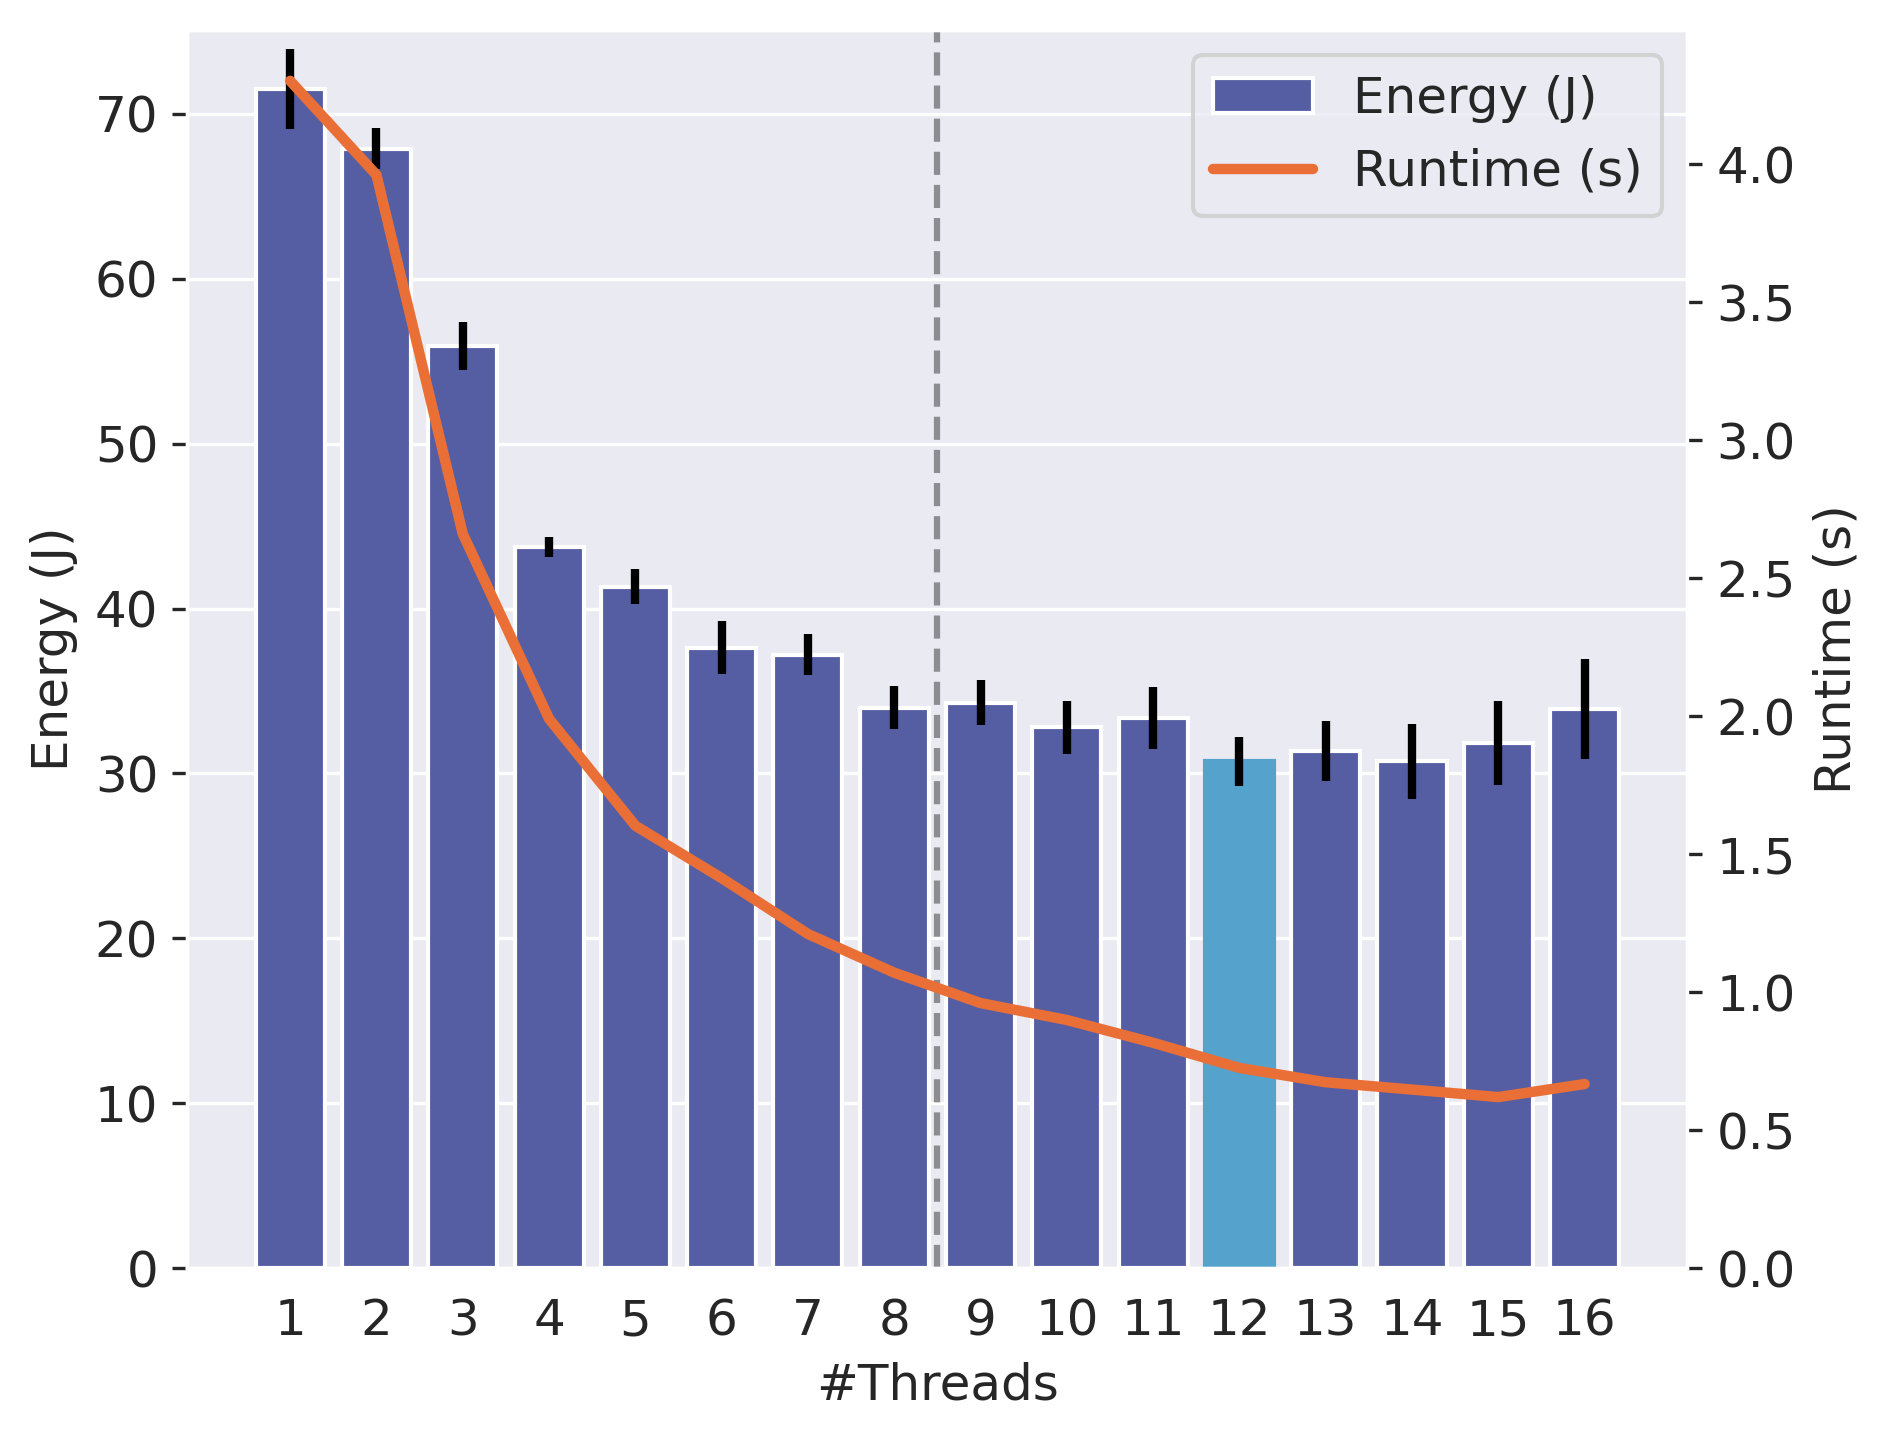
\includegraphics[width=\linewidth,alt={
            Chart showing energy consumption and runtime across different numbers of threads. The
            x-axis represents the number of threads from 1 to 16. The left y-axis shows bars
            indicating energy consumption in joules. The right y-axis shows an orange line
            indicating the runtime in seconds. Energy consumption peaks at one thread, and steadily
            decreases until roughly eight threads, after which it plateaus and reaches a minimum at
            12 threads. Runtime peaks at one thread, and gradually decreases until it plateaus
            around 12 threads.
        }]{images/nbody_40000.png}
        \caption{$40000$ elements.}
        \label{fig:nbody3}
    \end{subfigure}%
    \caption{Average energy consumption and runtime of 250 N-body simulation in SaC.
    Bars denote energy consumption, with corresponding values in the left y-axis.
    The line denotes runtime, corresponding to the right y-axis.}
    \label{fig:nbody}
\end{figure*}

\subsection{N-body simulation}
As our first benchmark we measure the energy consumption and runtime of a SaC implementation of
the N-body algorithm, given three different problem input sizes. The N-body algorithm is typically
applied in physics and astronomy to simulate the effect of physical sources, like gravity, on
systems of bodies such as particles and celestial objects. Each body is defined by a record type,
containing its current position, velocity, and mass. Although records in SaC use a similar
notation as in C, they are fully flattened into arrays of the record's fields, improving data
locality~\cite{sac-records}.

A single time step of the N-body simulation with delta-time \verb|dt| on an array of bodies is
defined as follows, where \verb|acc| is a function that returns the acceleration vector between two
bodies.
\begin{verbatim}
struct Body[n] nbody(struct Body[n] bodies, double dt)
{
    accel = { [i] -> sum({ [j] -> acc(bodies[i], bodies[j]) }) };
    bodies.pos += bodies.vel * dt;
    bodies.vel += accel * dt;
    return bodies;
}
\end{verbatim}

For these case studies only the relevant parallel codes are measured, namely the tensor
comprehensions. The runtime and energy measurements start right before those parallel regions, and
stop immediately after their synchronization. The average runtime and energy consumption for the
three input sizes are shown in Figure~\ref{fig:nbody}. Along the x-axis is the number of threads,
ranging from one to sixteen. Bars denote the average energy consumption of a single time step, and
the line denotes its average runtime.

For an N-body simulation with $10000$ elements in Figure~\ref{fig:nbody1} we observe that although
increasing the thread-count strictly decreases the runtime, for simulations with $25000$ and $40000$
elements in Figures~\ref{fig:nbody2} and \ref{fig:nbody3} respectively, the energy consumption
plateaus when using more than eight threads. It seems that any improvements in energy consumption
gained by using hyper-threading are mitigated by the energy overhead it introduces. Consequently, on
a system with shared resources and multiple running processes, it might be beneficial to select a
lower thread-count for the N-body simulation. This frees up the remaining threads to be used by
other processes, without incurring a significant negative energy consumption impact on the N-body
simulation. Although this increases the total runtime, it can conversely lead to energy savings.

An interesting observation, seen in the following benchmarks as well, is that increasing the
thread-count has a greater effect on runtime performance than on energy-efficiency. This suggests
that the overhead caused by having to manage multiple threads has a stronger negative effect on the
energy consumption of a program than on its runtime performance, and that optimizing for runtime
performance has diminishing returns for decreasing energy consumption.

\begin{figure*}[!ht]
    \centering
    \begin{subfigure}{0.33\linewidth}
        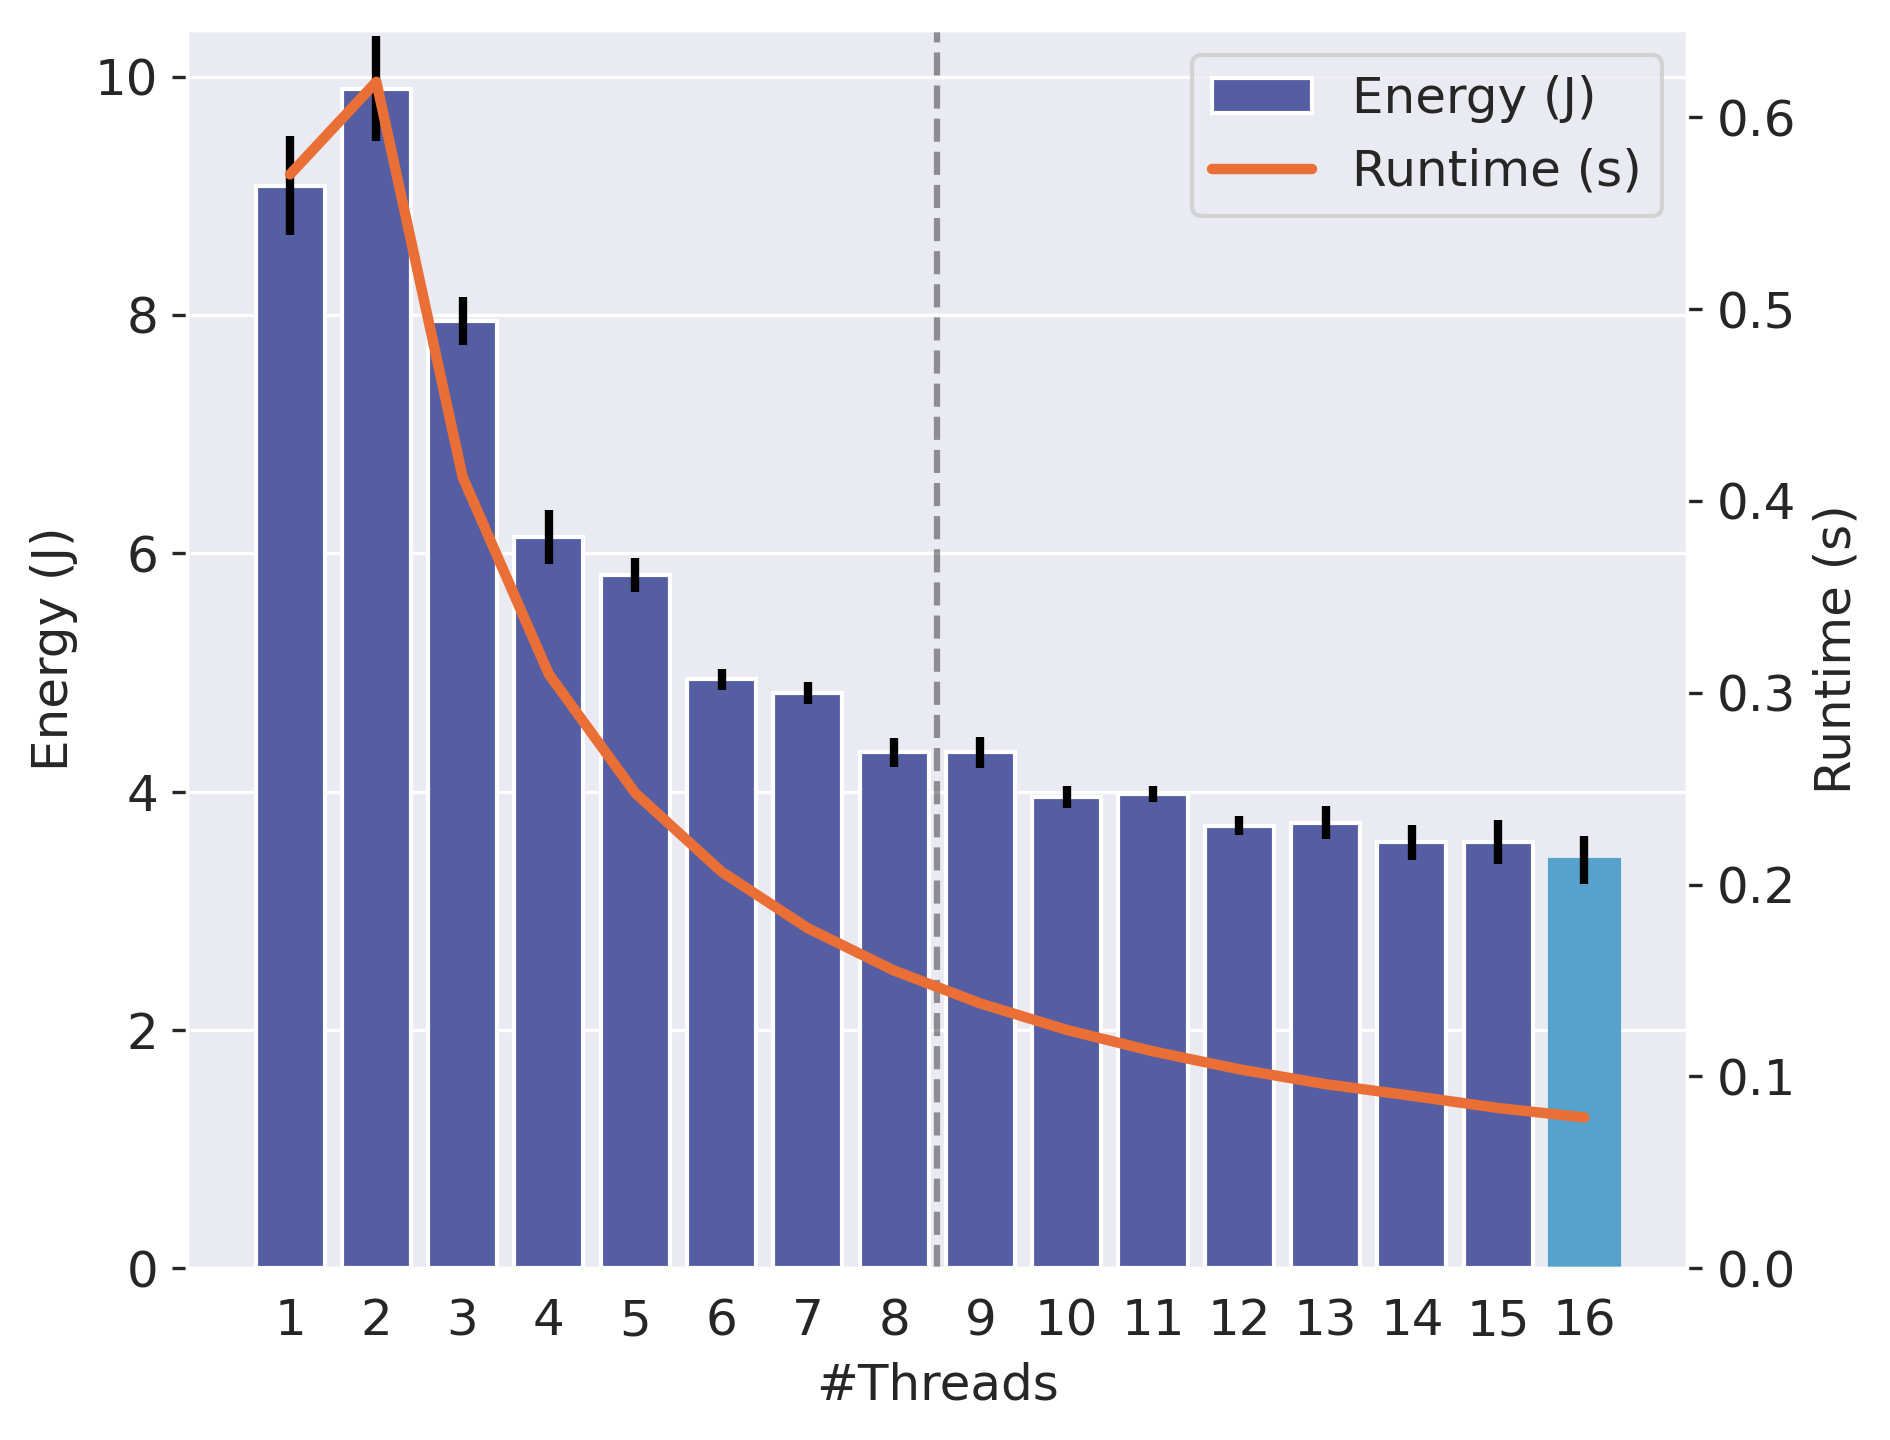
\includegraphics[width=\linewidth,alt={
            Chart showing energy consumption and runtime across different numbers of threads. The
            x-axis represents the number of threads from 1 to 16. The left y-axis shows bars
            indicating energy consumption in joules. The right y-axis shows an orange line
            indicating the runtime in seconds. Energy consumption peaks at two threads, and steadily
            decreases until roughly eight threads, after which it plateaus and reaches a minimum at
            16 threads. Runtime peaks at two threads, and gradually decreases until it reaches the
            minimum at 16 threads.
        }]{images/stencil_10000.png}
        \caption{$10000 \times 10000$ points.}
        \label{fig:stencil1}
    \end{subfigure}%
    \begin{subfigure}{0.33\linewidth}
        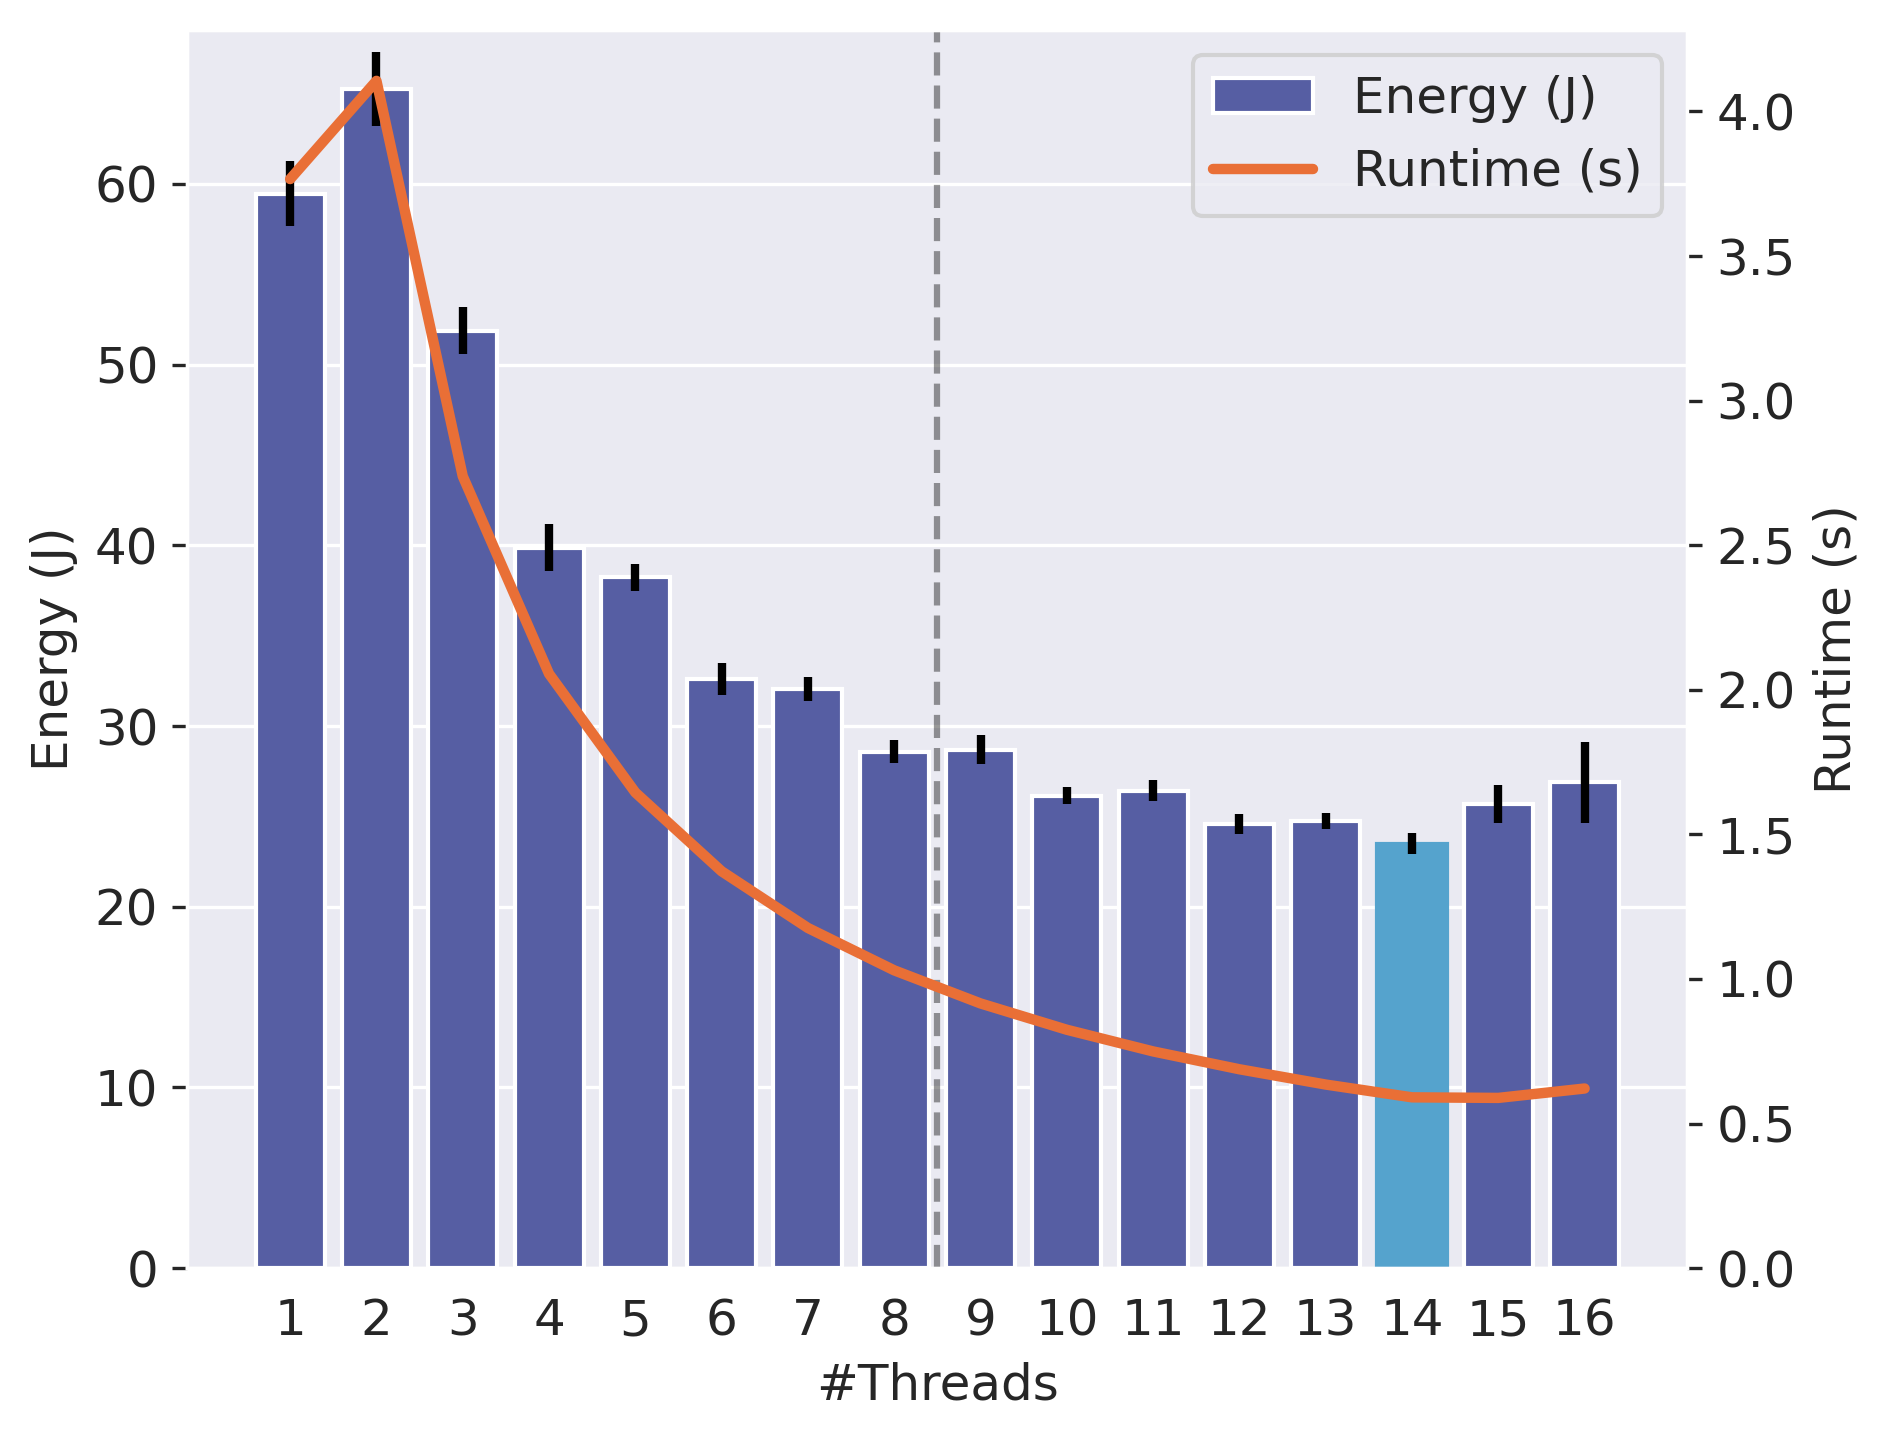
\includegraphics[width=\linewidth,alt={
            Chart showing energy consumption and runtime across different numbers of threads. The
            x-axis represents the number of threads from 1 to 16. The left y-axis shows bars
            indicating energy consumption in joules. The right y-axis shows an orange line
            indicating the runtime in seconds. Energy consumption peaks at two threads, and steadily
            decreases until roughly eight threads, after which it plateaus and reaches a minimum at
            14 threads. Runtime peaks at two threads, and gradually decreases until it plateaus
            around 14 threads.
        }]{images/stencil_25000.png}
        \caption{$25000 \times 25000$ points.}
        \label{fig:stencil2}
    \end{subfigure}%
    \begin{subfigure}{0.33\linewidth}
        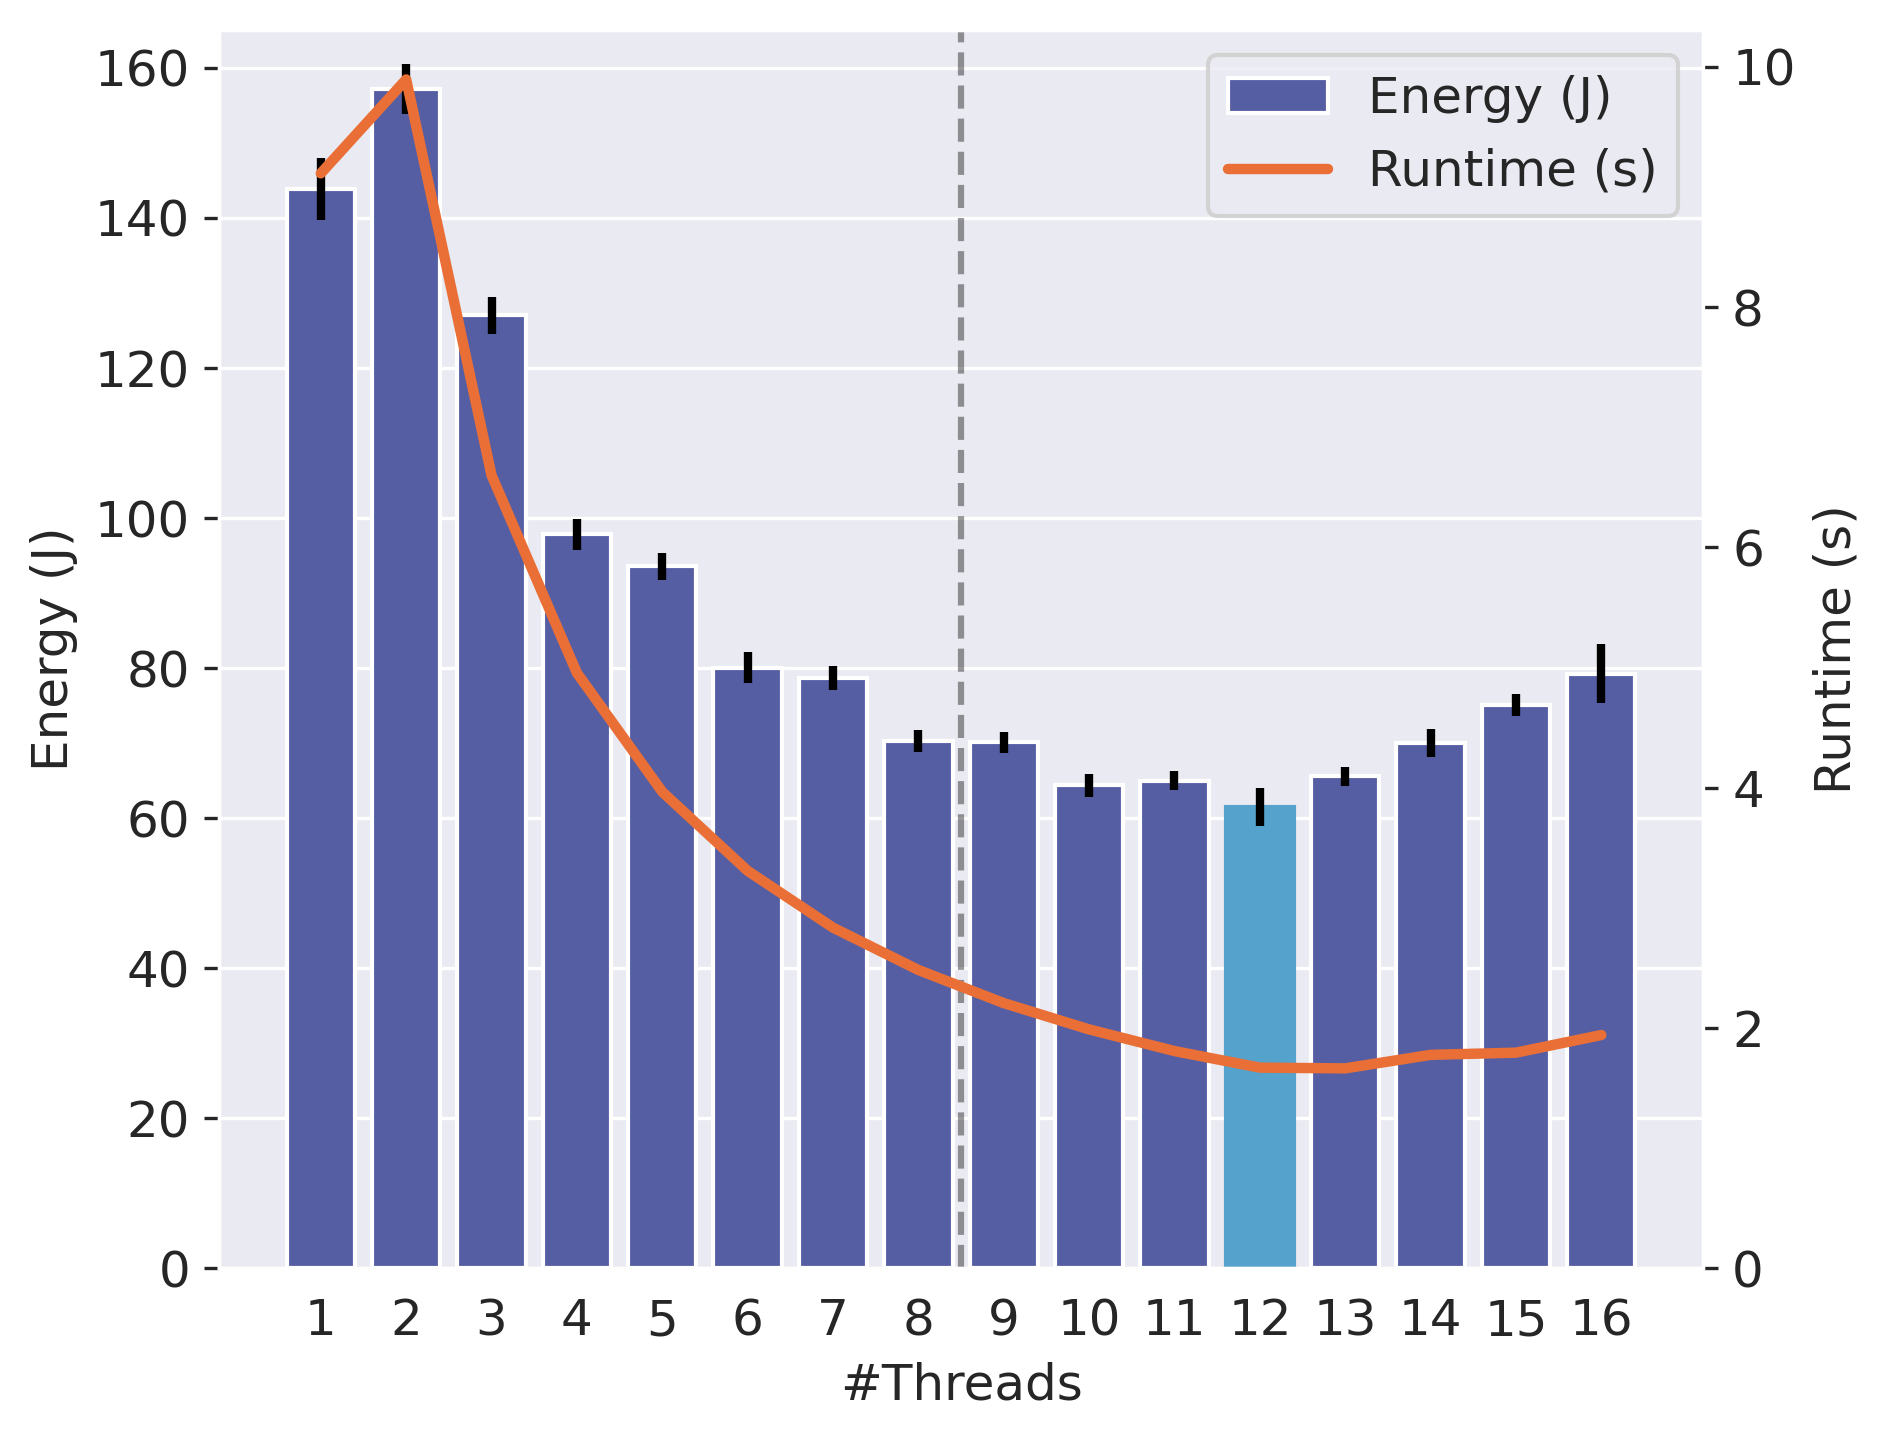
\includegraphics[width=\linewidth,alt={
            Chart showing energy consumption and runtime across different numbers of threads. The
            x-axis represents the number of threads from 1 to 16. The left y-axis shows bars
            indicating energy consumption in joules. The right y-axis shows an orange line
            indicating the runtime in seconds. Energy consumption peaks at two threads, and steadily
            decreases until roughly eight threads, after which it plateaus and reaches a minimum at
            12 threads. Runtime peaks at two threads, and gradually decreases until it plateaus
            around 12 threads.
        }]{images/stencil_40000.png}
        \caption{$40000 \times 40000$ points.}
        \label{fig:stencil3}
    \end{subfigure}%
    \caption{Average energy consumption and runtime of 250 nine-point stencil operations in SaC.
    Bars denote energy consumption, with corresponding values in the left y-axis.
    The line denotes runtime, corresponding to the right y-axis.}
    \label{fig:stencil}
\end{figure*}

\subsection{Nine-point stencil}\label{sec:stencil}
The nine-point stencil operation is used for image processing, computer simulations, and for solving
partial differential equations. Perhaps the most common application of the stencil operation
nowadays is in the training process of Convolutional Neural Networks~(CNN). In this context, the
stencil operation is applied for edge-detection and other image processing tasks, as well as for
providing a means for spatial awareness. Most relevant to us is the application of the stencil
operation for resizing arrays in CNNs, which highlights a real-world scenario where the input data
size changes during the runtime of a program.

The nine-point stencil is defined as a weighted sum of each point in an array and its eight
immediate neighbours, where each weight depends on the corresponding value in a $3 \times 3$ array
of weights. It is defined in SaC as:
\begin{verbatim}
double[2:shp] stencil(double[2:shp] arr, double[3,3] w)
{
    return { iv -> sum({ jv -> w[jv] * arr[mod(iv+jv-1, shp)] })
           | iv < shp };
}
\end{verbatim}

For a $10000 \times 10000$ input matrix in Figure~\ref{fig:stencil1} we observe that both the
runtime and energy consumption decrease as the number of threads increases. However, for $25000
\times 25000$ and $40000 \times 40000$ inputs, using all available threads is no longer optimal for
both the energy-efficiency and runtime performance. We see this in Figures~\ref{fig:stencil2} and
\ref{fig:stencil3} respectively, whereas the input size increases, the optimum thread-count
decreases.

\begin{figure*}[!ht]
    \centering
    \begin{subfigure}{0.33\linewidth}
        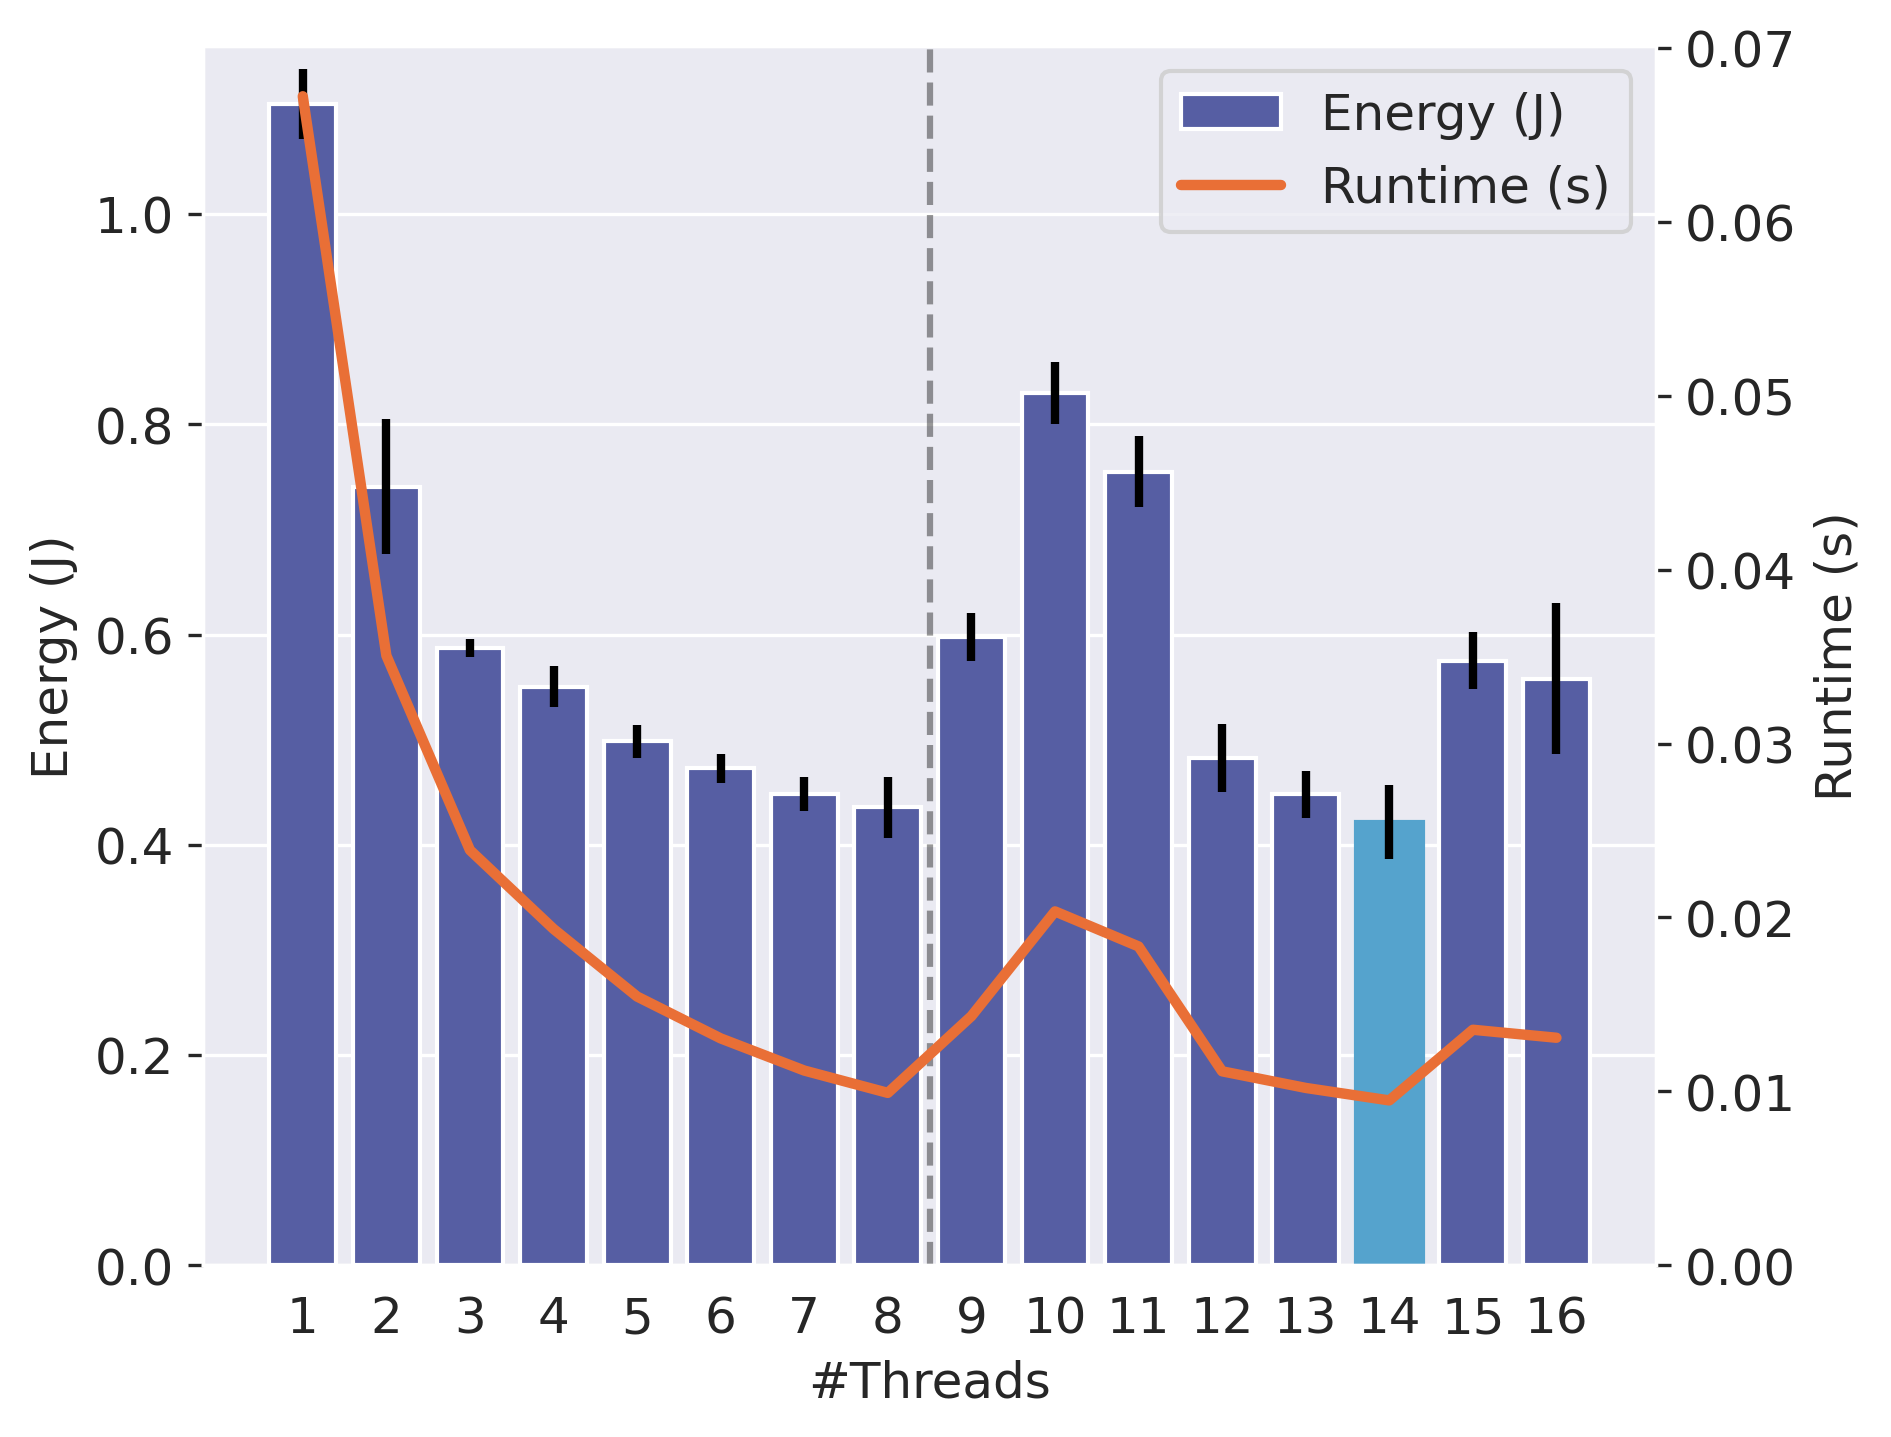
\includegraphics[width=\linewidth,alt={
            Chart showing energy consumption and runtime across different numbers of threads. The
            x-axis represents the number of threads from 1 to 16. The left y-axis shows bars
            indicating energy consumption in joules. The right y-axis shows an orange line
            indicating the runtime in seconds. Energy consumption peaks at one threads and gradually
            decreases from one to eight threads, after which it starts noticeably fluctuating.
            Reaching a minimum at 14 threads, with an energy consumption roughly equal to that of
            eight threads. Runtime follows a similar pattern, albeit being more pronounced.
        }]{images/matmul_500.png}
        \caption{$500 \times 500$ matrix.}
        \label{fig:matmul1}
    \end{subfigure}%
    \begin{subfigure}{0.33\linewidth}
        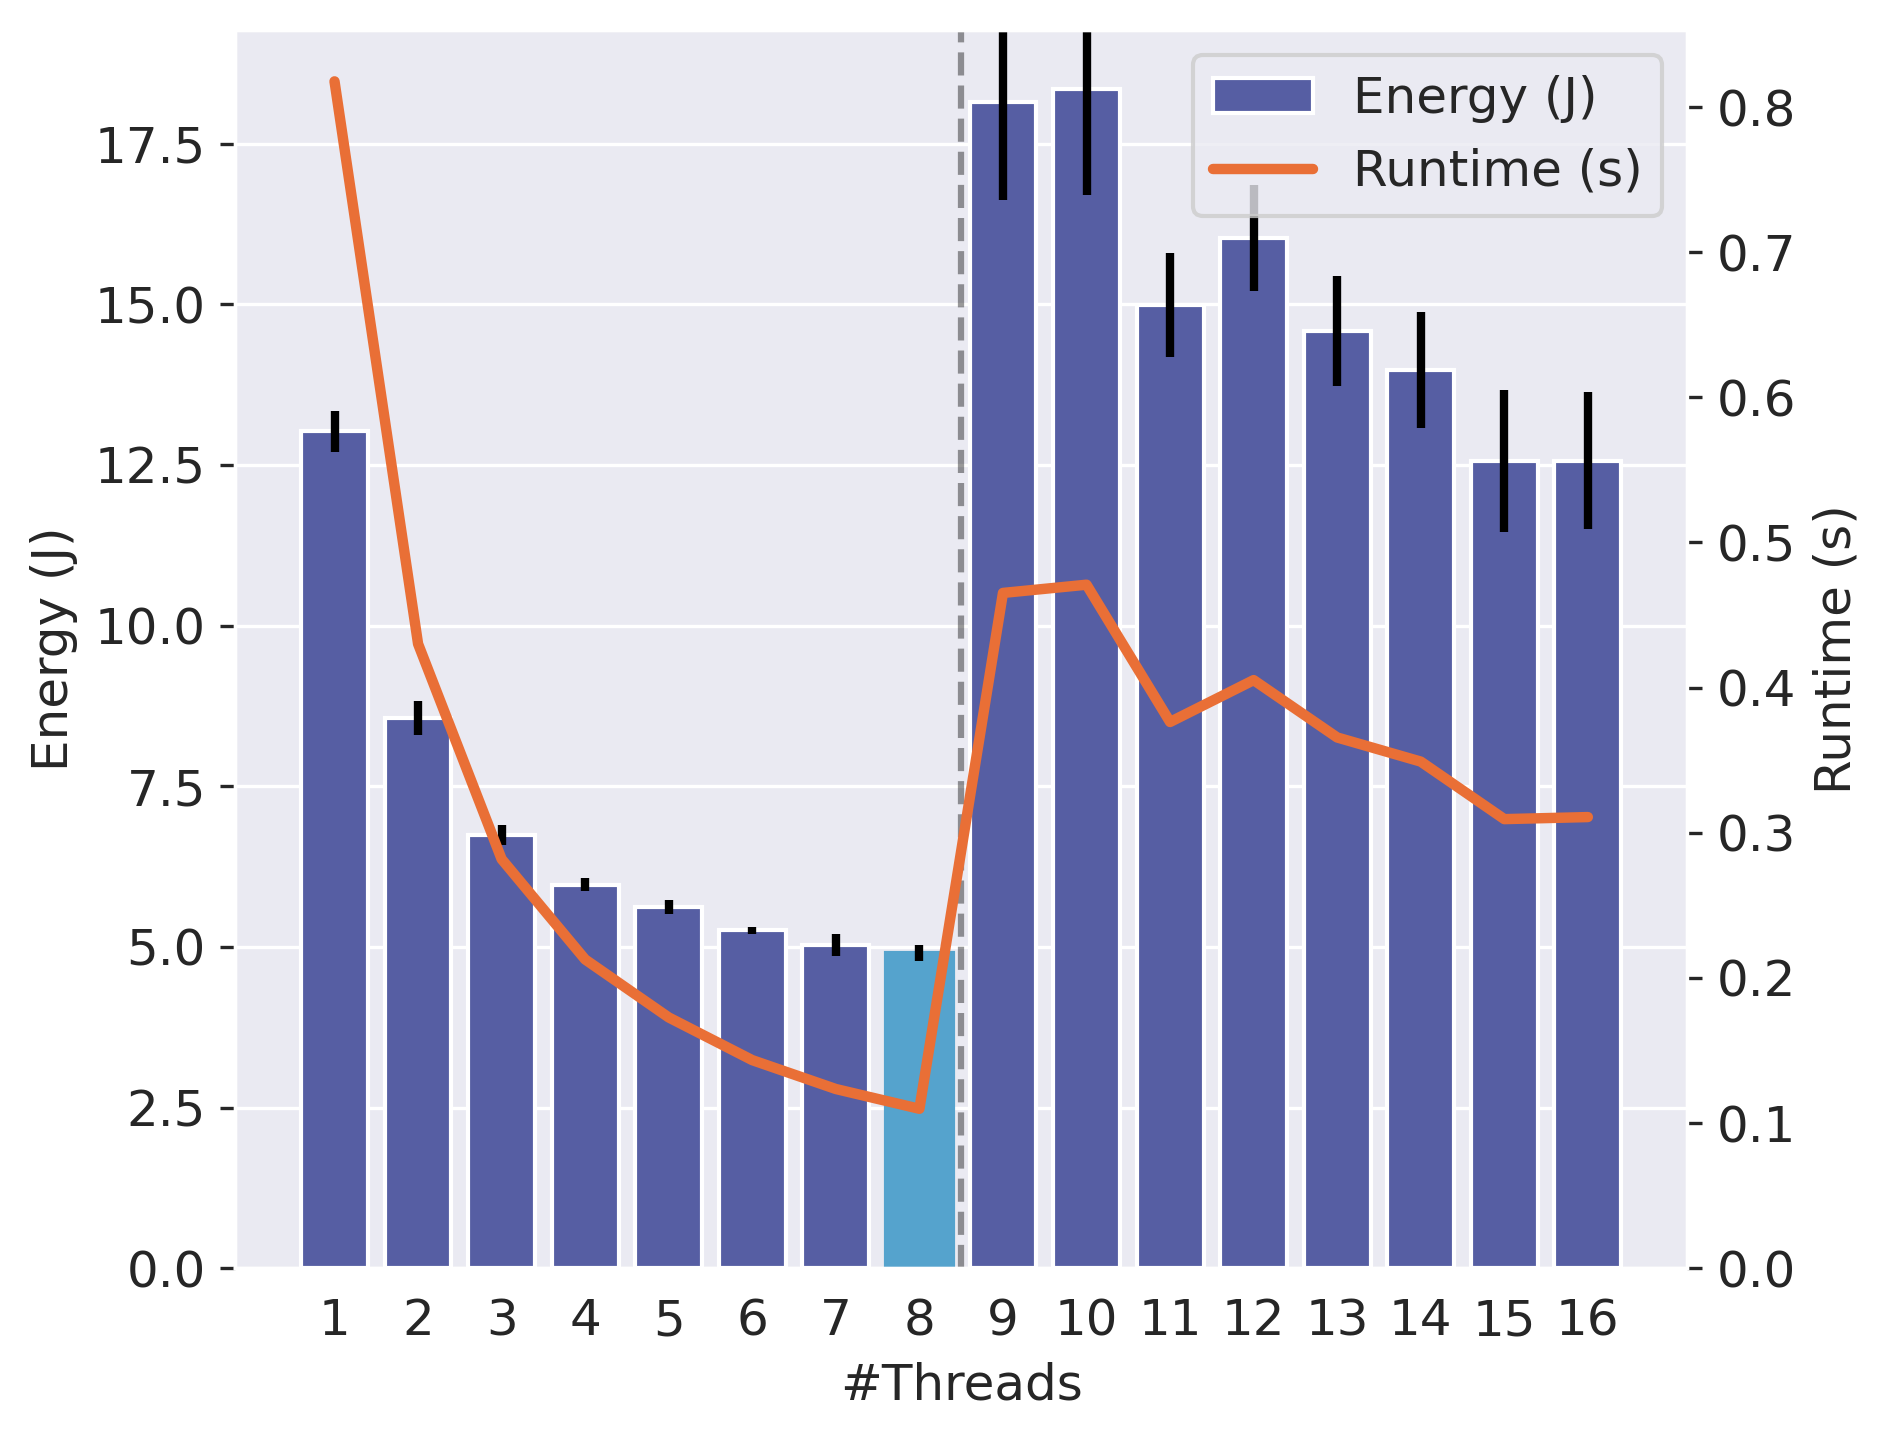
\includegraphics[width=\linewidth,alt={
            Chart showing energy consumption and runtime across different numbers of threads. The
            x-axis represents the number of threads from 1 to 16. The left y-axis shows bars
            indicating energy consumption in joules. The right y-axis shows an orange line
            indicating the runtime in seconds. Energy consumption gradually decreases from one to
            eight threads, reaching a minimum at eight threads. Going to nine threads there is a
            significant jump in energy consumption, peaking at nine threads and gradually decreasing
            until 16 threads. The energy consumption of 16 threads is above that of one thread.
            Runtime follows a similar pattern, albeit being more pronounced.
        }]{images/matmul_1000.png}
        \caption{$1000 \times 1000$ matrix.}
        \label{fig:matmul2}
    \end{subfigure}%
    \begin{subfigure}{0.33\linewidth}
        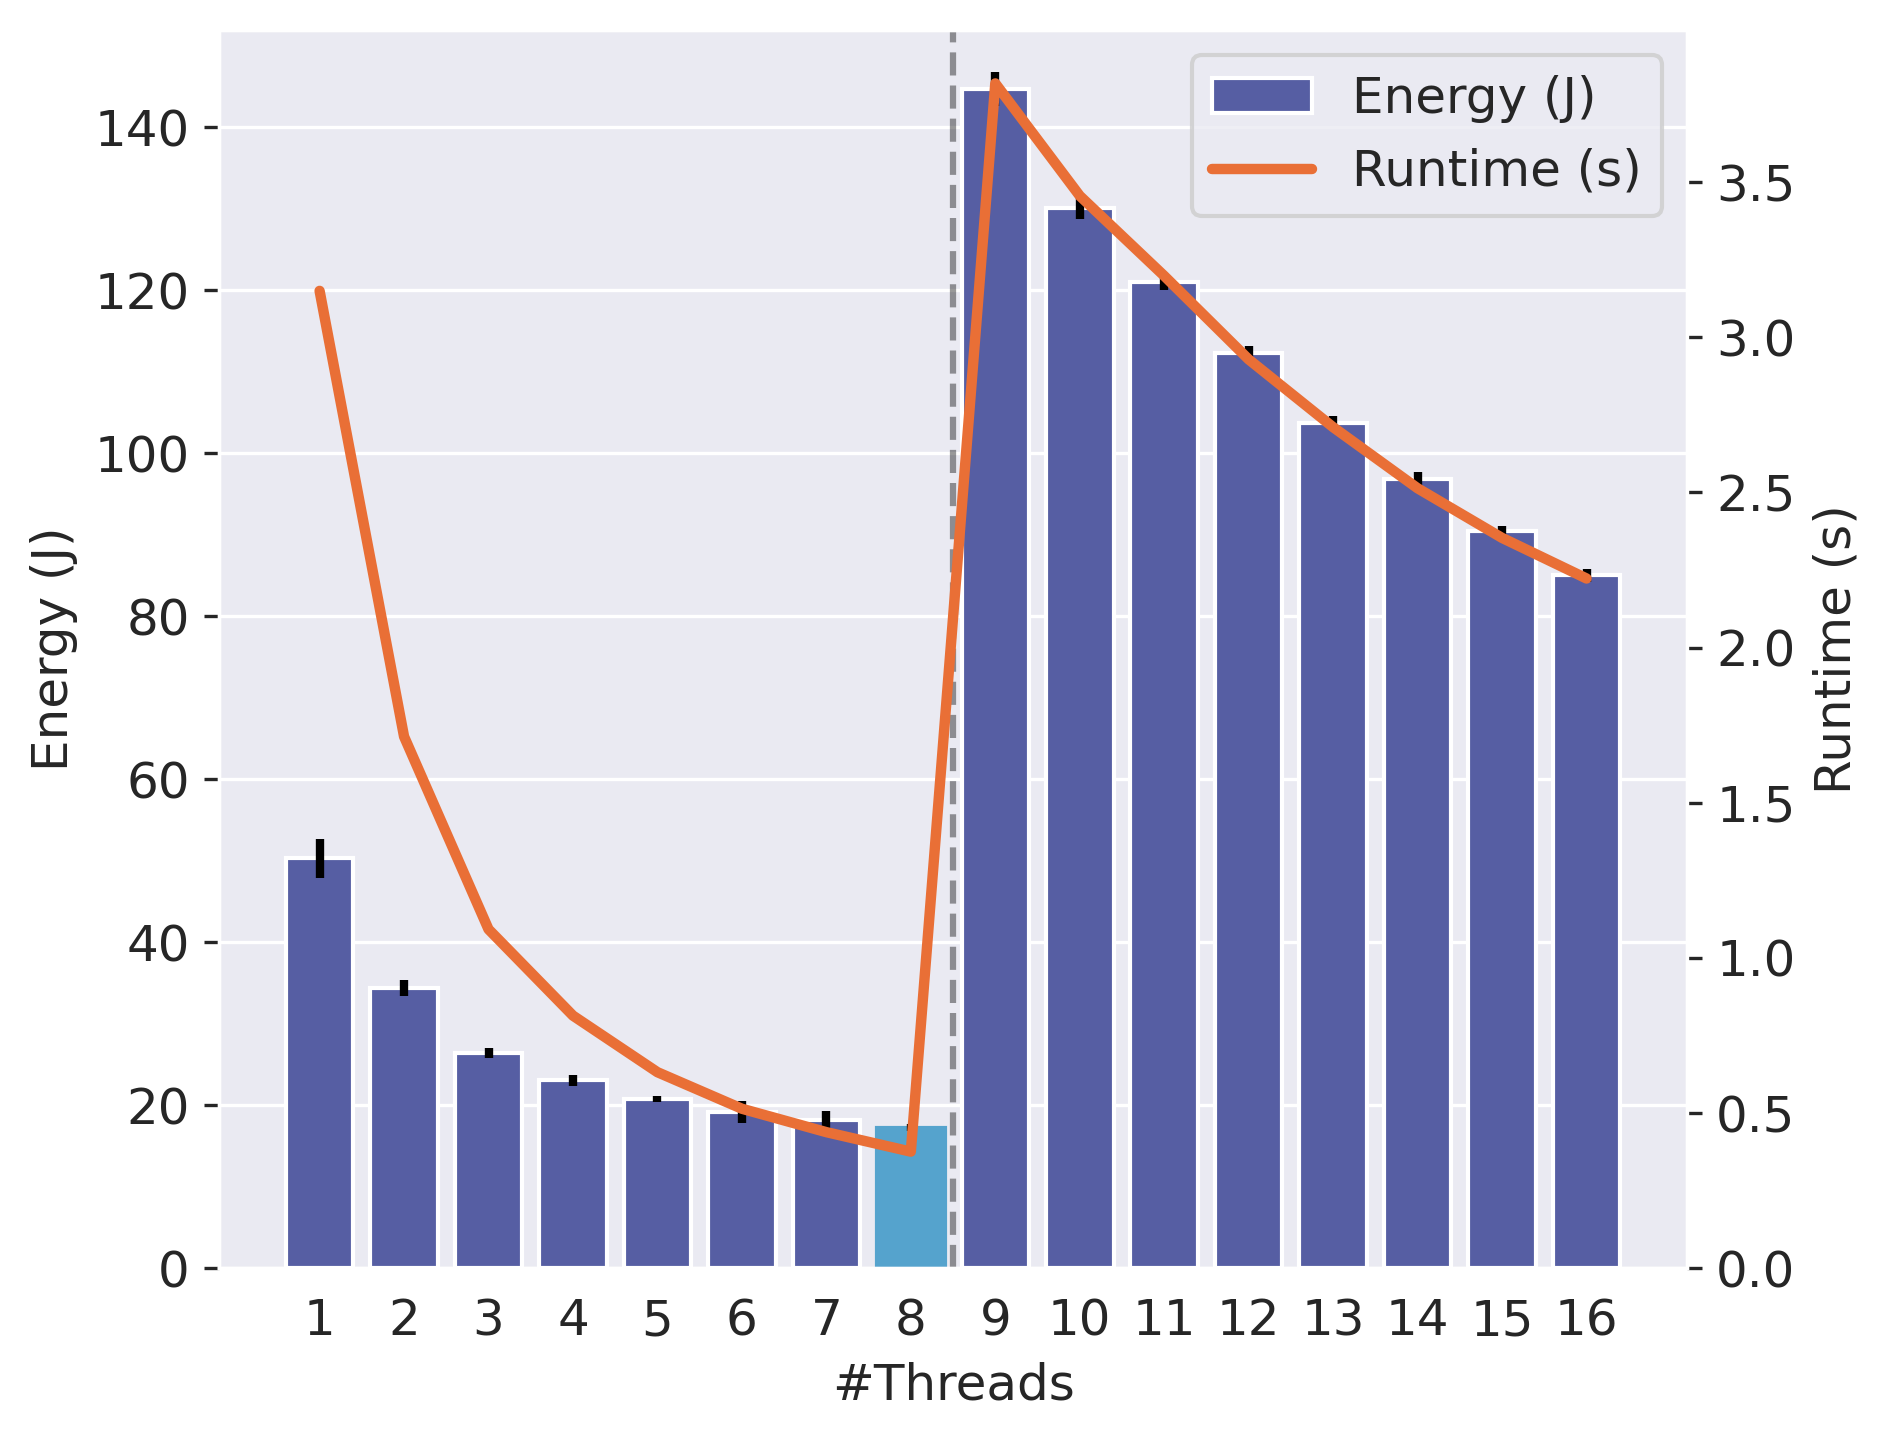
\includegraphics[width=\linewidth,alt={
            Chart showing energy consumption and runtime across different numbers of threads. The
            x-axis represents the number of threads from 1 to 16. The left y-axis shows bars
            indicating energy consumption in joules. The right y-axis shows an orange line
            indicating the runtime in seconds. Energy consumption gradually decreases from one to
            eight threads, reaching a minimum at eight threads. Going to nine threads there is a
            significant jump in energy consumption, peaking at nine threads and gradually decreasing
            until 16 threads. The energy consumption of 16 threads is above that of one thread.
            Runtime follows a similar pattern, albeit being more pronounced.
        }]{images/matmul_1500.png}
        \caption{$1500 \times 1500$ matrix.}
        \label{fig:matmul3}
    \end{subfigure}%
    \caption{Average energy consumption and runtime of 250 naive matrix multiplications in SaC.
    Bars denote energy consumption, with corresponding values in the left y-axis.
    The line denotes runtime, corresponding to the right y-axis.}
    \label{fig:matmul}
\end{figure*}

\subsection{Matrix multiplication}
The matrix multiplication algorithm is used across a variety of domains, from solving linear
equations, to machine learning, to computer graphics. Whereas more sophisticated approaches aim to
have consistent cache locality~\cite{sac-blocking}, the cache locality of the naive approach
decreases as the input size increases, shifting the bottleneck from CPU to memory. We implement the
naive algorithm, since this behaviour provides us with an interesting case study.

The SaC implementation closely resembles the mathematical definition:
\begin{verbatim}
double[u,w] matmul(double[u,v] a, double[v,w] b)
{
    return { [i,j] -> sum({ [k] -> a[i,k] * b[k,j] }) };
}
\end{verbatim}

Due to cache behaviour of the naive implementation, manual tuning is required to ensure an efficient
thread layout. When using eight or fewer threads, an interleaved mode is optimal, ensuring each
thread executes on a different physical core. However, since the system only has eight physical
cores, using nine or more threads requires multi-threading. At this point an interleaved mode is no
longer beneficial as it increases the amount of false sharing, drastically decreasing performance.
It should be noted that choosing a different thread pinning strategy leads to significantly
different observations, and that choosing an efficient thread layout is crucial to the performance
of this benchmark.

The results of a $500 \times 500$ matrix multiplication in Figure~\ref{fig:matmul1} align with our
expectations; increasing the number of threads up to eight threads improves both the
energy-efficiency and the runtime performance. Using more threads causes a decrease in performance,
likely due to additional thread management overhead. This overhead is somewhat overcome by the
increase in thread-count, making a thread-count of fourteen threads similar in performance to a
thread-count of eight. However, as observed in Figures~\ref{fig:matmul2} and \ref{fig:matmul3},
increasing the matrix size to $1000 \times 1000$ and $1500 \times 1500$ changes this energy
consumption pattern, resulting from the shift of being CPU-bound to being memory-bound. Even with an
efficient thread pinning strategy, using more than eight threads causes a significant increase in
both the energy consumption and runtime, making those approaches worse for energy-efficiency than
even a single-threaded approach.

\begin{figure*}[!ht]
    \centering
    \begin{subfigure}{0.33\linewidth}
        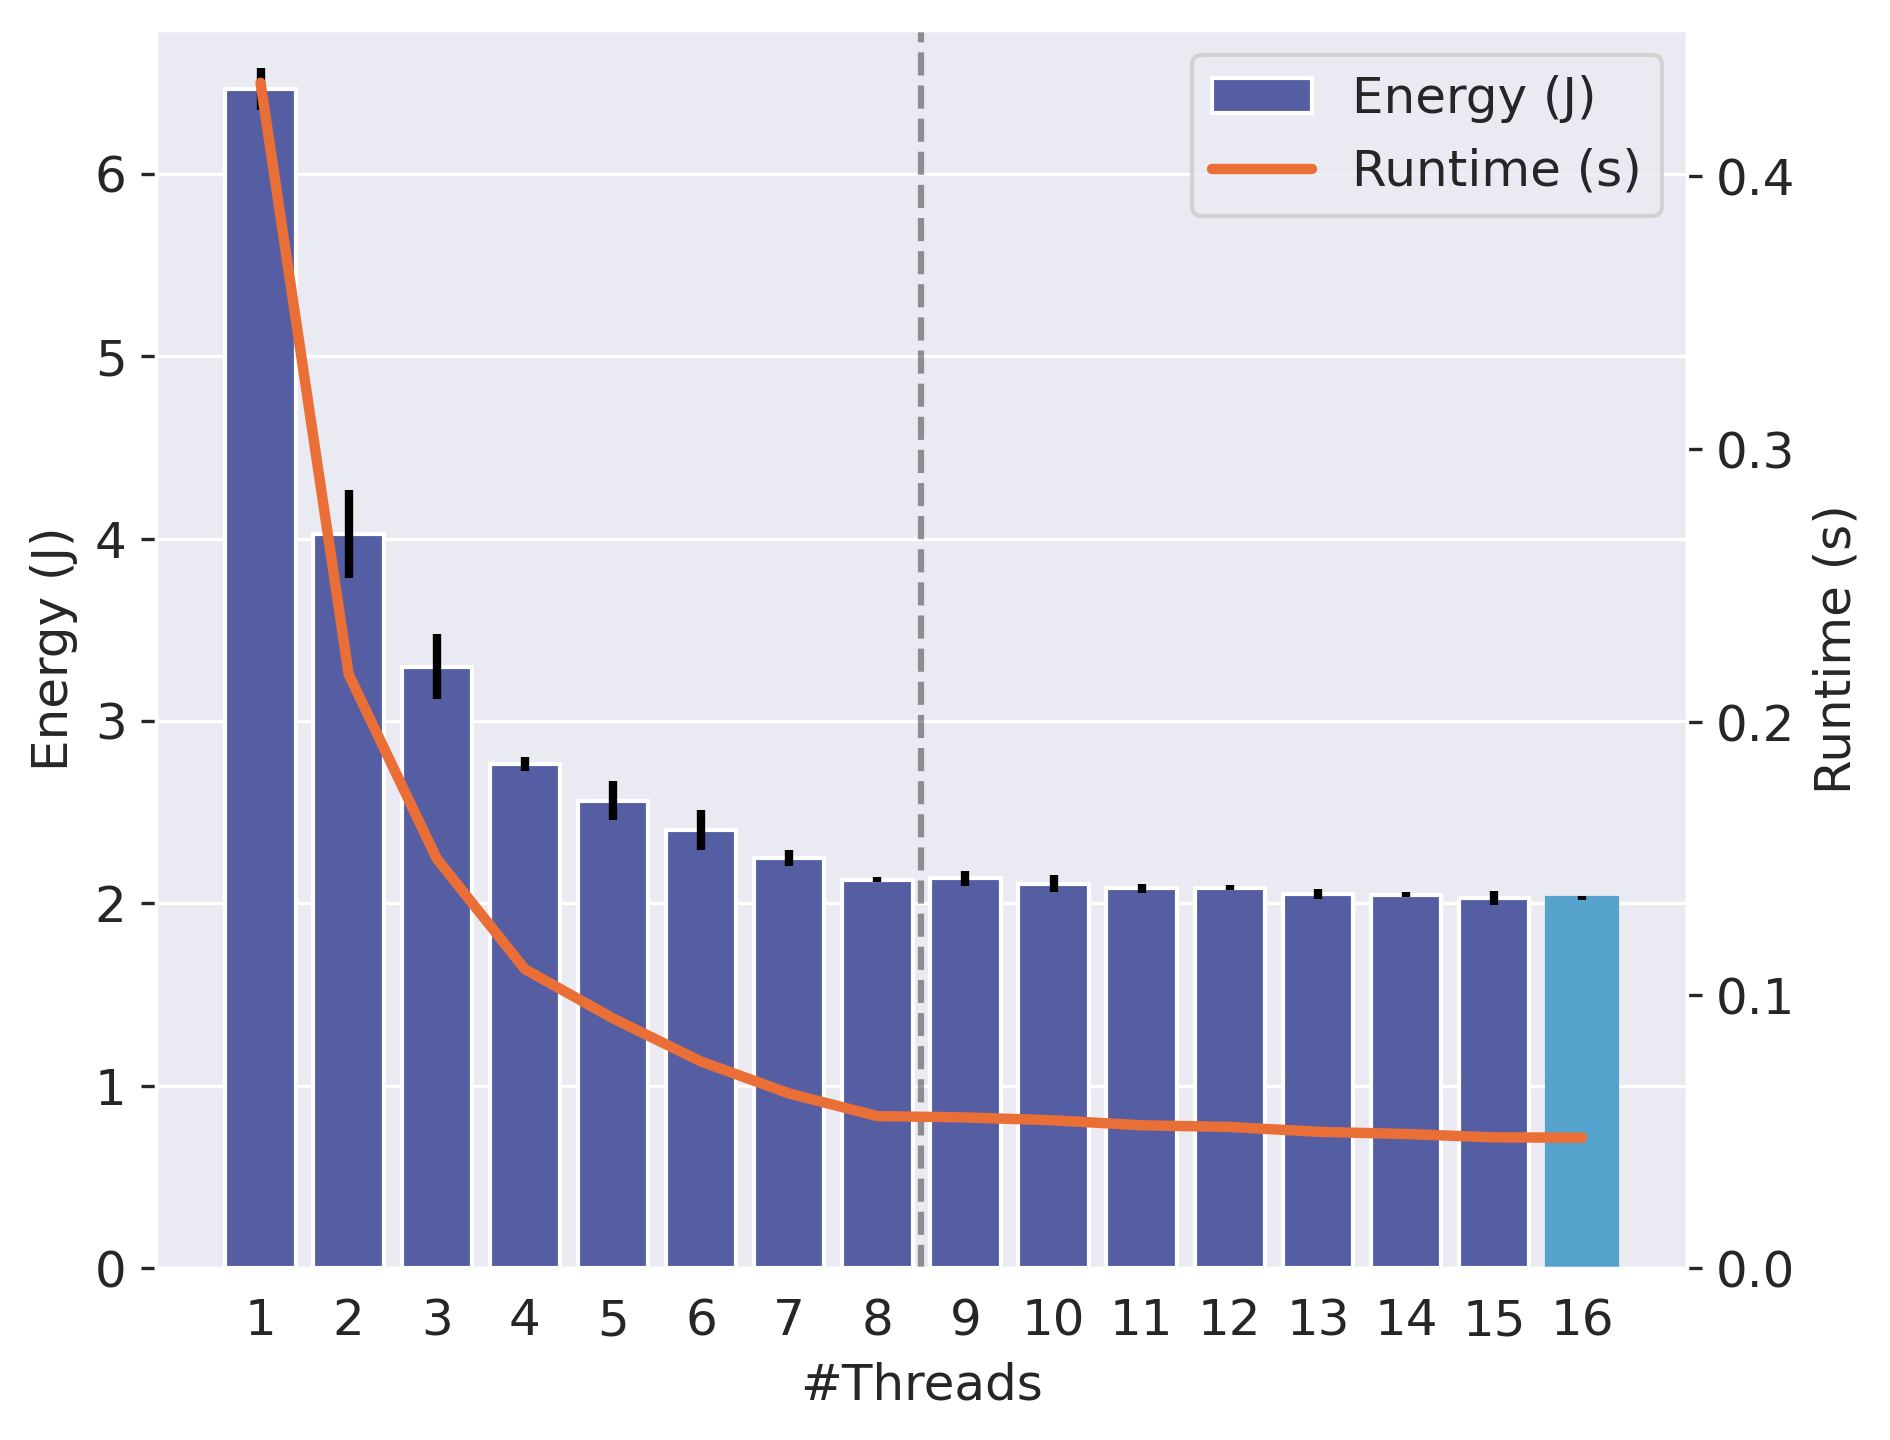
\includegraphics[width=\linewidth,alt={
            Chart showing energy consumption and runtime across different numbers of threads. The
            x-axis represents the number of threads from 1 to 16. The left y-axis shows bars
            indicating energy consumption in joules. The right y-axis shows an orange line
            indicating the runtime in seconds. Energy consumption peaks at one threads, and steadily
            decreases until roughly eight threads, after which it plateaus and reaches a minimum at
            16 threads. Runtime follows the same pattern.
        }]{images/rust_500.png}
        \caption{$500 \times 500$ matrix.}
        \label{fig:rust1}
    \end{subfigure}%
    \begin{subfigure}{0.33\linewidth}
        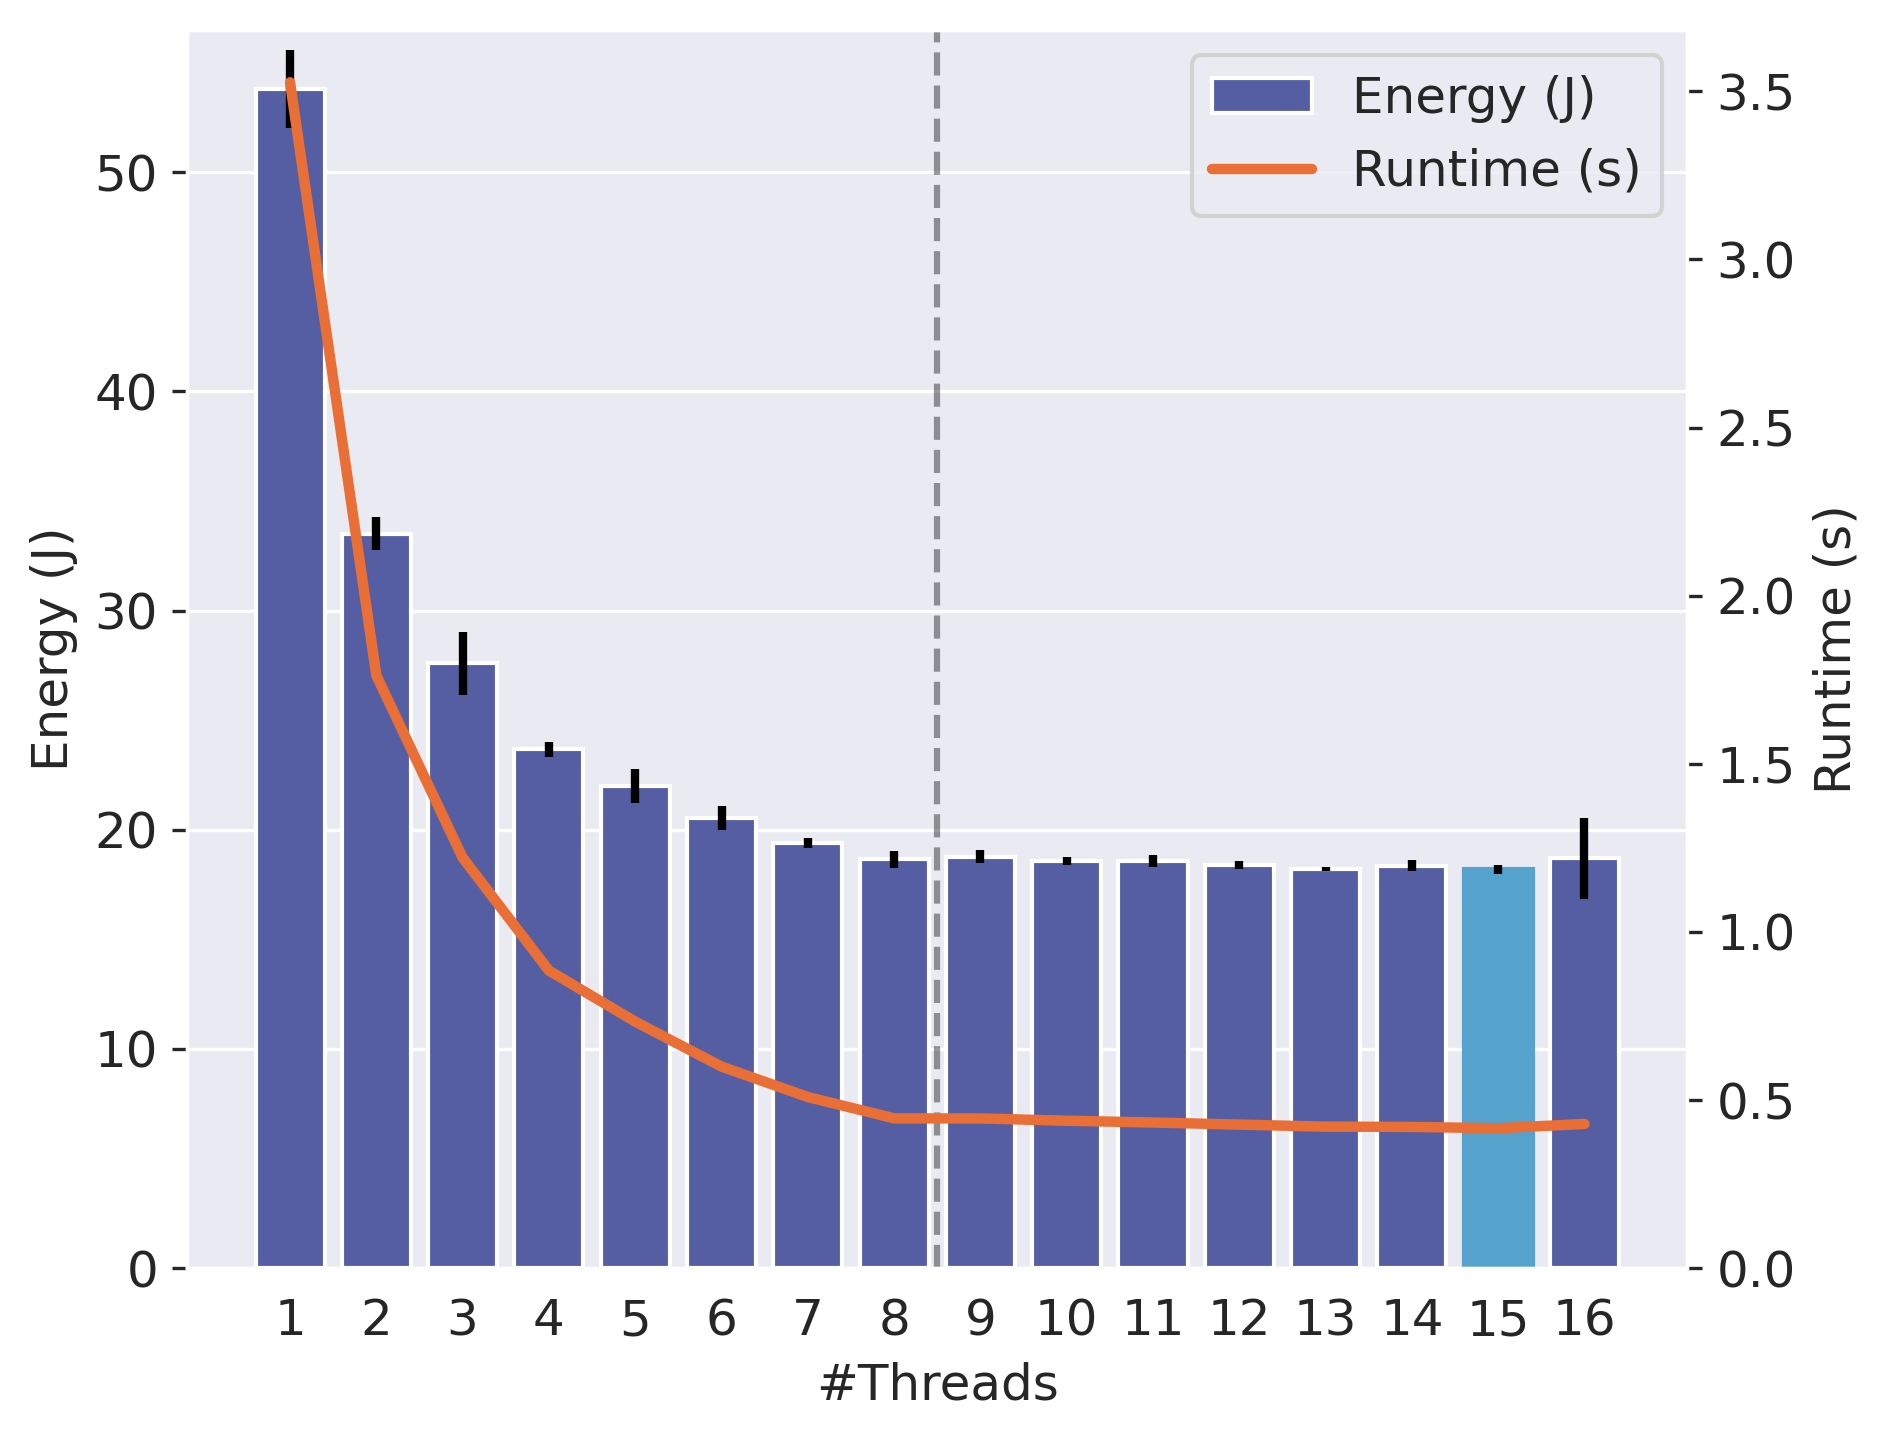
\includegraphics[width=\linewidth,alt={
            Chart showing energy consumption and runtime across different numbers of threads. The
            x-axis represents the number of threads from 1 to 16. The left y-axis shows bars
            indicating energy consumption in joules. The right y-axis shows an orange line
            indicating the runtime in seconds. Energy consumption peaks at one threads, and steadily
            decreases until roughly eight threads, after which it plateaus and reaches a minimum at
            15 threads. Runtime follows the same pattern.
        }]{images/rust_1000.png}
        \caption{$1000 \times 1000$ matrix.}
        \label{fig:rust2}
    \end{subfigure}%
    \begin{subfigure}{0.33\linewidth}
        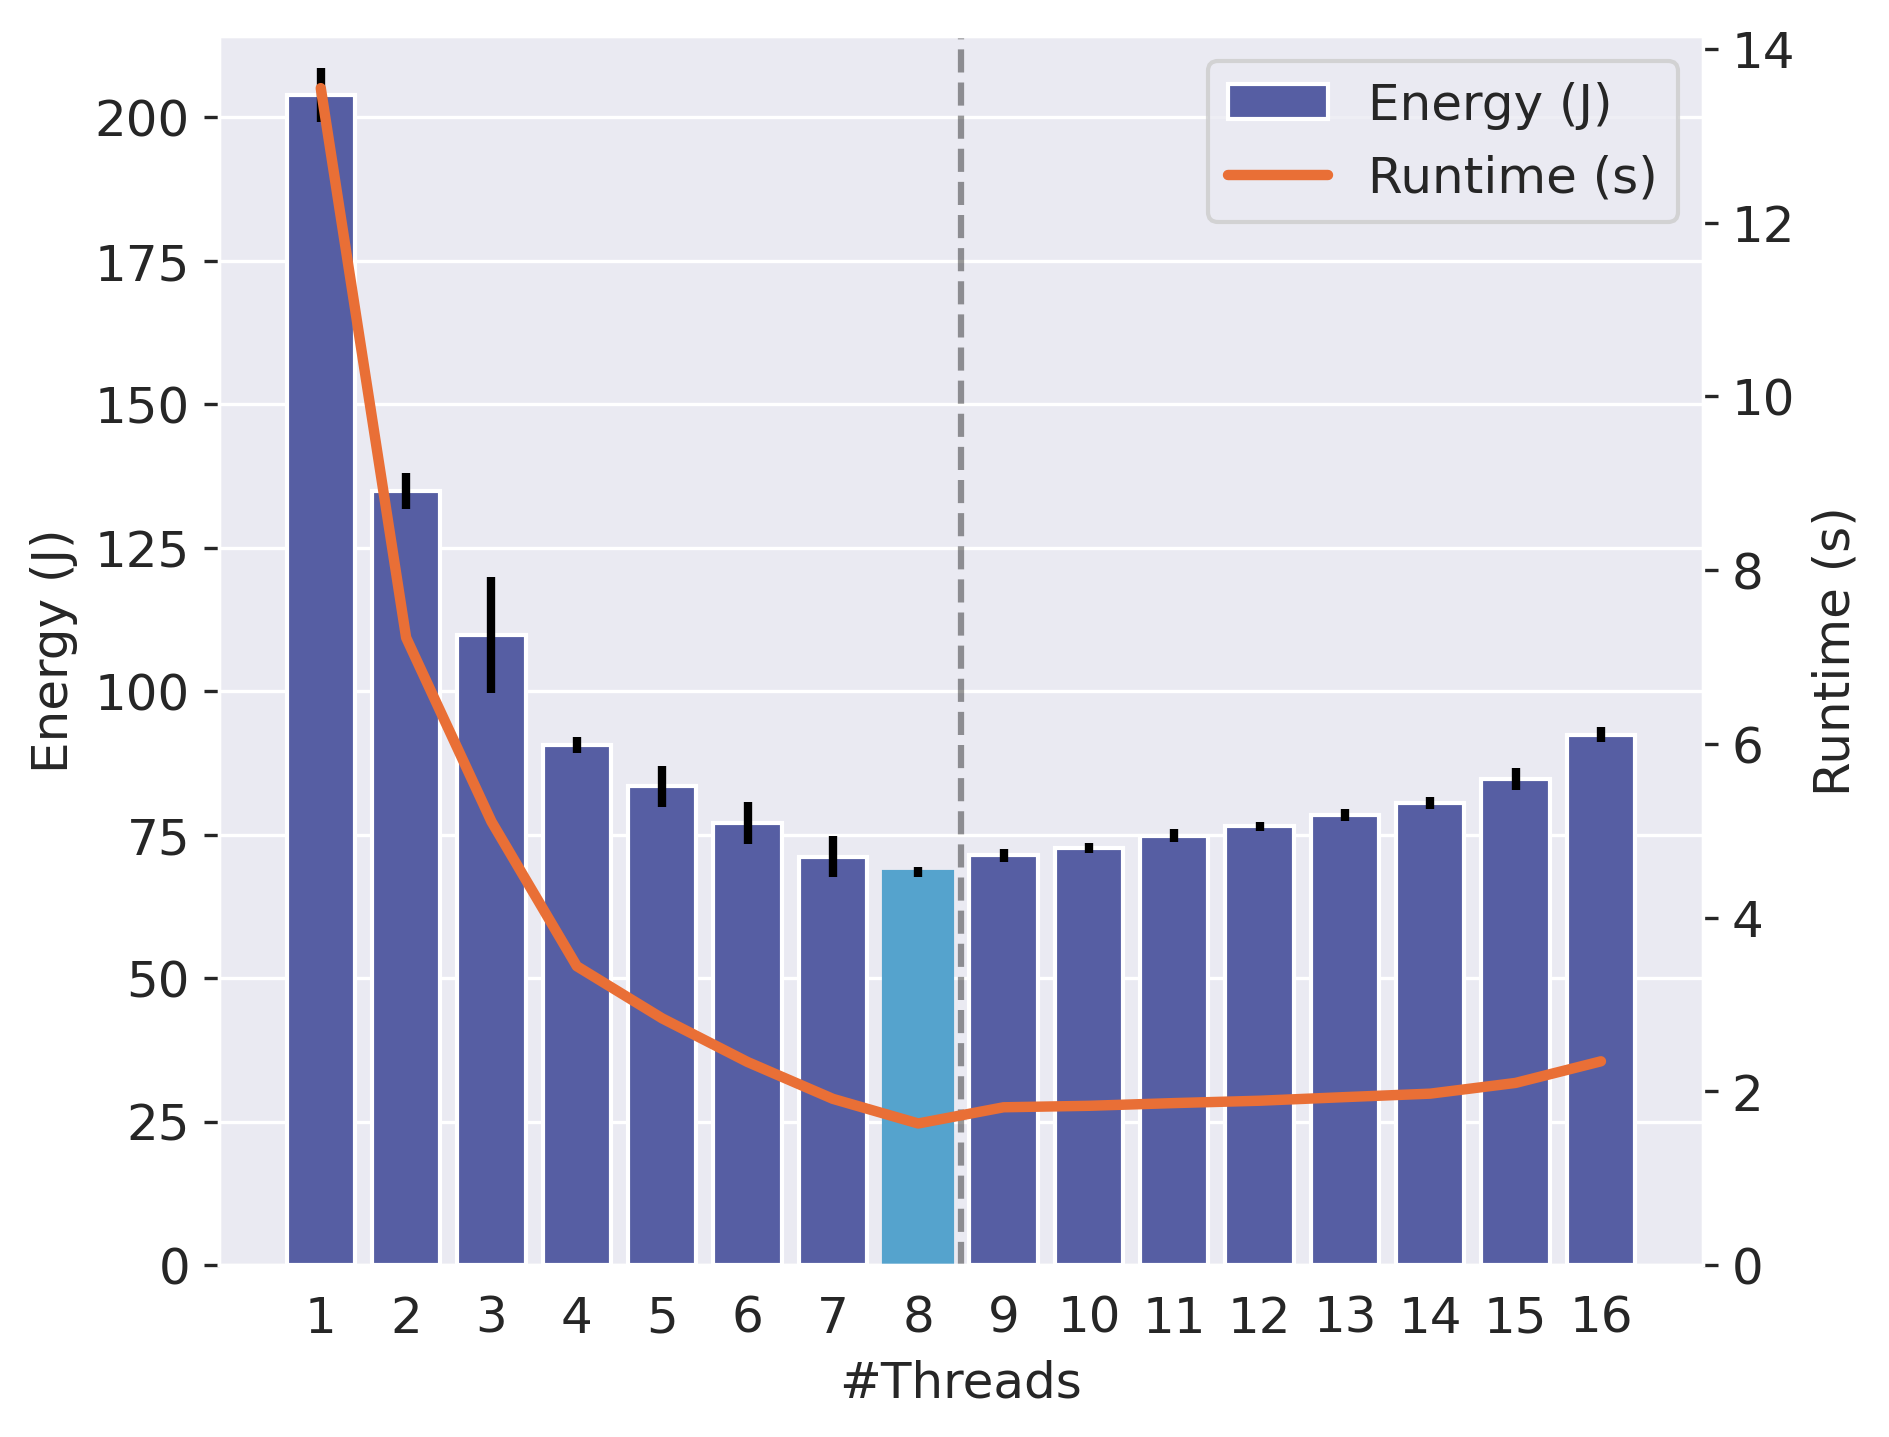
\includegraphics[width=\linewidth,alt={
            Chart showing energy consumption and runtime across different numbers of threads. The
            x-axis represents the number of threads from 1 to 16. The left y-axis shows bars
            indicating energy consumption in joules. The right y-axis shows an orange line
            indicating the runtime in seconds. Energy consumption peaks at one threads, and steadily
            decreases until it reaches a minimum at eight threads, after which energy consumption
            starts gradually increasing again. Runtime follows the same pattern.
        }]{images/rust_1500.png}
        \caption{$1500 \times 1500$ matrix.}
        \label{fig:rust3}
    \end{subfigure}%
    \caption{Average energy consumption and runtime of 250 naive matrix multiplications in Rust.
    Bars denote energy consumption, with corresponding values in the left y-axis.
    The line denotes runtime, corresponding to the right y-axis.}
    \label{fig:rust}
\end{figure*}

\subsection{Implementation language}
To validate that these observations are not specific to SaC, we also evaluate a manually
parallelized implementation of the matrix multiplication algorithm in Rust. We observe in
Figure~\ref{fig:rust} that switching the implementation language from SaC to Rust produces a
significantly different energy consumption pattern. In Figures~\ref{fig:rust1} and \ref{fig:rust2}
we observe that up until eight threads, increasing the thread-count improves both the
energy-efficiency and runtime. When using more than eight threads, both the energy consumption and
runtime plateau, suggesting that we gain no additional benefits by using hyper-threading. As the
matrix size increases to $1500 \times 1500$, there is a shift in the energy consumption pattern. As
the number of threads increases from 8 to 16, the energy consumption gradually increases again. This
suggests that the overhead associated with hyper-threading outweighs the benefits of further
parallelization.

Interestingly, although the SaC and Rust implementations provide a similar level of performance
when using nine or more threads, comparing the best-case scenarios we find that the SaC
implementation performs roughly four times better in terms of energy consumption and roughly five
times better in terms of runtime. As discussed previously, thread pinning and cache behaviour have a
significant impact on the performance characteristics of this benchmark. Although we suspect that
these are the main reasons for this performance difference, it is unclear why exactly this behaviour
occurs, complicating the task of determining an optimal thread-count and emphasizing the need for a
dynamic approach.
